\documentclass[review]{elsarticle}

\usepackage{hyperref}
\usepackage{lineno}
\modulolinenumbers[5]
\usepackage{amsmath}
\usepackage{graphicx}
\usepackage{booktabs}
\usepackage{url}
\usepackage{caption}
\usepackage{siunitx}
\usepackage{geometry}
\usepackage{multirow}
\usepackage{listings}
\usepackage{csvsimple}
\usepackage[T1]{fontenc}
\usepackage{hyphenat}
% \usepackage{underscore} % not needed; causes conflicts
\usepackage{enumitem}
\usepackage{prisma-flow-diagram}
\usepackage{placeins}

% PDF metadata and link styling
\hypersetup{
  colorlinks=true,
  linkcolor=blue,
  citecolor=blue,
  urlcolor=blue,
  pdftitle={WS3: An open-source Python framework for integrated simulation and optimization of forest landscape and wood supply systems},
  pdfauthor={Gregory Paradis},
  pdfsubject={Submitted to Ecological Informatics},
  pdfkeywords={WS3, wood supply, forest estate, forest planning, optimization, libCBM, carbon accounting, environmental modelling, Python}
}

\newcommand{\woodstocknum}[1]{\num[round-mode=places,round-precision=2]{#1}}
\newif\ifwoodstockParityLoaded
\woodstockParityLoadedfalse
\newcommand{\loadWoodstockParity}{%
  % Defaults ensure compilation if CSV is unavailable
  \global\def\woodstockHarvestAreaWS{0}%
  \global\def\woodstockHarvestAreaWoodstock{0}%
  \global\def\woodstockHarvestAreaDiff{0}%
  \global\def\woodstockHarvestVolumeWS{0}%
  \global\def\woodstockHarvestVolumeWoodstock{0}%
  \global\def\woodstockHarvestVolumeDiff{0}%
  \global\def\woodstockStockWS{0}%
  \global\def\woodstockStockWoodstock{0}%
  \global\def\woodstockStockDiff{0}%
  \IfFileExists{tables/woodstock_parity.csv}{%
    \woodstockParityLoadedtrue
    \csvreader[head to column names]{tables/woodstock_parity.csv}{metric=\metricname,ws3_value=\wsvalue,woodstock_value=\woodstockvalue,percent_diff=\percentdiff}{%
      \ifcsvstrcmp{\metricname}{total_harvest_area_ha}{%
        \global\edef\woodstockHarvestAreaWS{\wsvalue}%
        \global\edef\woodstockHarvestAreaWoodstock{\woodstockvalue}%
        \global\edef\woodstockHarvestAreaDiff{\percentdiff}%
      }{%
        \ifcsvstrcmp{\metricname}{total_harvest_volume_m3}{%
          \global\edef\woodstockHarvestVolumeWS{\wsvalue}%
          \global\edef\woodstockHarvestVolumeWoodstock{\woodstockvalue}%
          \global\edef\woodstockHarvestVolumeDiff{\percentdiff}%
        }{%
          \ifcsvstrcmp{\metricname}{total_growing_stock_m3}{%
            \global\edef\woodstockStockWS{\wsvalue}%
            \global\edef\woodstockStockWoodstock{\woodstockvalue}%
            \global\edef\woodstockStockDiff{\percentdiff}%
          }{}%
        }%
      }%
    }%
  }{}
}

\journal{Ecological Informatics}

\begin{document}

\begin{frontmatter}

\title{WS3: An open-source Python framework for integrated simulation and optimization of forest landscape and wood supply systems}

\author[ubc]{Gregory Paradis\corref{cor1}}
\cortext[cor1]{Corresponding author: gregory.paradis@ubc.ca}
\address[ubc]{Faculty of Forestry, University of British Columbia, Canada}

% Graphical abstract (optional)
\begin{graphicalabstract}
  \centering
  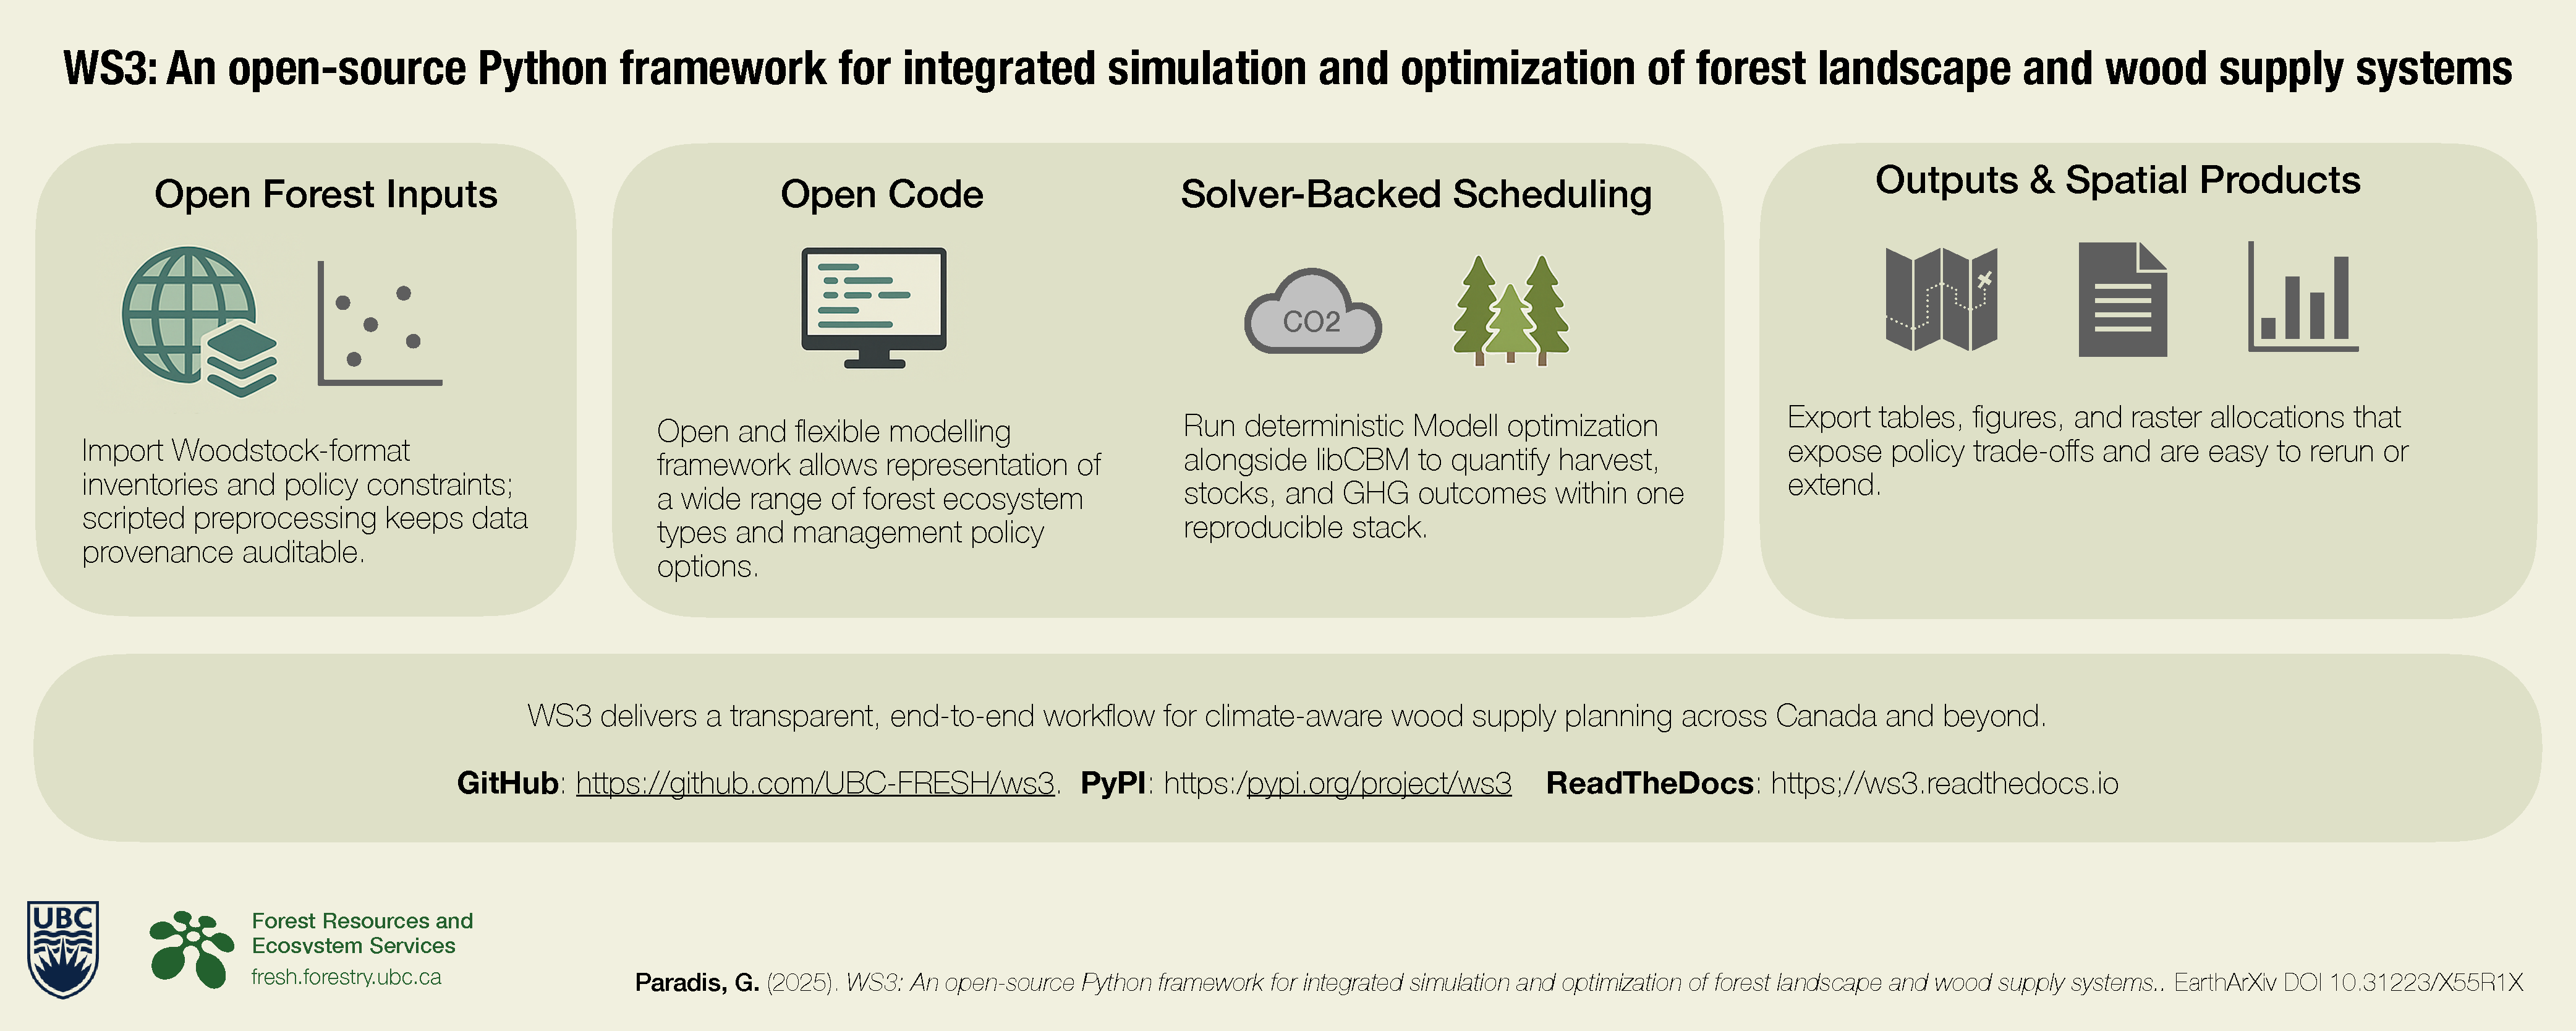
\includegraphics[width=\linewidth]{ws3-manuscript-graphical-abstract.pdf}
\end{graphicalabstract}

\section*{Highlights}
\begin{itemize}
  \item Open-source Python framework for forest estate decision support.
  \item Solver-agnostic Model I generator with parallel LP build.
  \item Native libCBM linkage for carbon stock and flux accounting.
  \item Hybrid aspatial-to-raster workflows with reproducible geospatial I/O.
  \item Deterministic reproduction package and archived scaling benchmarks.
\end{itemize}

\begin{abstract}
Transparent decision support for forest landscapes demands integrated scheduling, carbon accounting, and spatial reporting. WS3 is an open-source Python framework that unifies modular simulation, solver-backed Model~I optimization, and raster allocation in a single, scriptable workflow aimed at reproducible ecological analyses. The system ingests Woodstock-style inventories, actions, and scenarios; exposes an explicit data model; and automates aspatial--spatial conversions so planners can move directly from harvest schedules to georeferenced disturbance footprints. Native linkage to the Canadian Forest Service Carbon Budget Model (libCBM) provides carbon stock and flux estimates for Canada and other libCBM-calibrated jurisdictions while preserving the transparency required for regulatory review.

The manuscript makes three contributions to ecological informatics. First, it documents a modular software architecture that decouples inventory ingestion, linear-programming harvest scheduling, carbon bookkeeping, and raster allocation, enabling users to mix heuristics and solver-backed approaches, swap solvers (PuLP/HiGHS or Gurobi), and extend indicators without rewriting the workflow. Second, it validates the framework through a parity analysis against a Woodstock industrial benchmark (differences \(<1\%\) across harvested volume, area, and growing stock) and through computational scaling experiments that expose runtime and memory envelopes from desktop to multi-core high-performance computing environments. Third, it releases the complete toolchain---source code, configuration files, and deterministic reproduction scripts---under the MIT license with an archived Zenodo DOI, ensuring that figures, tables, and diagnostic statistics can be rebuilt end-to-end.

We showcase WS3 on three British Columbia landscapes covering 2--5 million m\(^3\) of standing volume per site. Alternative objective sets (volume maximization, harvest area minimization, ecosystem carbon maximization, and net emissions minimization) reveal the expected trade-offs between volume and carbon outcomes while quantifying impacts on jobs, revenue, and spatial footprint. Carbon trajectories generated via libCBM illustrate how mitigation-focused schedules preserve ecosystem stocks and delay harvest emissions, whereas volume-oriented schedules deliver higher short-term flows at the expense of increased net emissions. Raster allocation routines produce wall-to-wall disturbance footprints that can be consumed by SpaDES-based cumulative-effects models or shared directly with rights-holders. The reproduction suite includes notebooks, container-ready scripts, and pinned dependency manifests so practitioners can adapt the workflow to their own inventories, run scaling benchmarks, and verify solver parity against their existing pipelines.

By lowering the technical barrier to open, auditable forest planning, WS3 enables agencies, industry, Indigenous governments, and researchers to co-develop climate-aligned harvest strategies, evaluate fuel-management or nature-based-solution scenarios, and couple harvest schedules with broader ecological simulations. The framework provides a reusable informatics scaffold for decision-making under competing sustainability mandates and supports rapid experimentation in emerging carbon-accounting and ecosystem-service policies.
\end{abstract}

\begin{keyword}
computational ecology \sep decision support \sep forest planning \sep optimization \sep carbon accounting \sep geospatial workflows
\end{keyword}

\section*{Software availability}
\begin{itemize}
  \item Software name: WS3 (Wood Supply Simulation System)
  \item Developer and contact: Gregory Paradis (Faculty of Forestry, University of British Columbia); \href{mailto:gregory.paradis@ubc.ca}{gregory.paradis@ubc.ca}
  \item First public release and current version: 2015 (v0.1); current release v1.0.5
  \item Programming language and dependencies: Python (>=3.9); optional extras include \texttt{libcbm\_py}, PuLP/HiGHS, and Gurobi
  \item Source repository and issue tracker: \url{https://github.com/UBC-FRESH/ws3}
  \item Distribution channel: PyPI package \texttt{ws3} (\texttt{pip install ws3} or \texttt{ws3[cbm]}) with wheels for Linux, macOS, and Windows
  \item Documentation: \url{https://ws3.readthedocs.io}
  \item Archived release: Zenodo DOI \href{https://doi.org/10.5281/zenodo.17331213}{10.5281/zenodo.17331213}
  \item License: MIT
  \item Hardware and OS requirements: Linux, macOS, or Windows; tested on Ubuntu 24.04 and macOS 14; CPU-only with recommended 16+ GB RAM for large LP instances
  \item Tested Python versions: 3.9--3.12 (continuous-integration matrix)
  \item Data form and access: supplementary CSV, GeoTIFF, and notebook artifacts packaged in the GitHub repository and Zenodo release; total archive size < 50 MB excluding optional outputs
\end{itemize}

\end{frontmatter}

\clearpage

\linenumbers

\section{Introduction}

Forested landscapes now sit at the centre of intertwined climate mitigation, biodiversity, and bioeconomy mandates, and planners are being asked to reconcile wood supply security with measurable reductions in greenhouse-gas emissions across multi-decadal horizons \citep{canadell2022wgiii, griscom2017natural, fao2020fra}. Meeting these expectations demands decision-support systems that can span harvest scheduling, regeneration and silviculture options, spatial footprint analysis, and explicit carbon accounting, all while remaining transparent enough for regulators, Indigenous governments, and industrial partners to audit \citep{law2018land, smyth2020climate}. The resulting analytical load has outgrown the ad hoc spreadsheets and siloed software stacks still common in practice, underscoring the need for integrated modelling platforms that support reproducible workflows and uphold emerging open-science norms such as the PERFICT principles for predictive ecology \citep{hampton2015tao, lowndes2017path, mcintire2022perfict}.

Strategic forest planning has long relied on operations-research formulations such as Model~I path scheduling and its variants, which underpin allowable-cut analyses and forest estate studies worldwide \citep{johnson1977techniques, gunn2007models, gunn2009some, paradis2013risk}. In practice these ideas are delivered through proprietary toolchains---Woodstock, Patchworks, JLP (MELA), and Heureka among others---that package data models, solvers, and reporting inside closed desktop environments \citep{remsoft-woodstock, patchworks, jlp_mela, heureka}. Historically, FPS-Atlas offered similar functionality but, as a proprietary product, is no longer distributed or maintained \citep{fps_atlas}. While these systems are mature and widely trusted, their licensing, opaque configuration formats, and limited automation support constrain transparency, collaborative extension, and reproducible research workflows increasingly required by regulators and journals \citep{hampton2015tao}.

In response, an open-source ecosystem has begun to chip away at these constraints. Spatial simulation platforms such as SpaDES and LANDIS-II, scenario-management frameworks like SyncroSim, and integrative planning prototypes such as PRISM demonstrate strong community appetite for modular, shareable tooling \citep{spades, landisii, syncrosim, nguyen2022prism}. SpaDES in particular mirrors WS3's open-science commitments---the core team helped write the PERFICT guidance---yet, by design, it delivers a coordination shell that depends on user-supplied simulation modules for every landscape process. That architecture excels at orchestrating high-fidelity spatial and stochastic dynamics, but the developers themselves acknowledge that harvest modules rarely move beyond stylised heuristics. They have therefore started collaborating with us on a \texttt{spades\_ws3} wrapper so SpaDES users can bring professional-grade wood-supply scheduling into cumulative-effects experiments. LANDIS-II and SELES occupy similar ecological-simulation niches but remain harder to adapt for rigorous forest-estate analysis: LANDIS-II's governance, C\# codebase, and Windows-centric binaries slow outside contributions and impede deployment to linux-based cloud or high-performance computing (HPC) environments, while SELES is closed-source black-box commercial software whose advanced modules typically require direct support from its original developer. In practice, practitioners must still bolt on their own solver integrations, carbon-accounting pipelines, and spatial reporting to assemble a full decision-support stack \citep{daigneault2022forest, law2018land}. Parallel efforts such as the French CAPSIS platform illustrate both the promise and the effort required to host interoperable forest growth models: CAPSIS underpins climate-sensitive planning experiments \citep{fortin2022altframework} and Bayesian meta-modelling work for Quebec landscapes \citep{fortin2022metamodel}, and it remains the delivery vehicle for the ARTEMIS stem-level growth model used by the Quebec government to generate official hardwood yield curves \citep{power2015artemis}. These international experiences align with broader calls for interoperable, climate-sensitive growth modelling ecosystems capable of linking models across scales \citep{gilson2025climatesensitive}. This persistent gap between open landscape-simulation scaffolds and purpose-built forest-estate planning motivates the deterministic, optimization-first framework we introduce with WS3 in the following section.

WS3 fills this methodological gap with a fully open Python framework that preserves the expressive power of legacy Model~I scheduling while embedding reproducibility, automation, and carbon accounting as first-class design goals. It imports Woodstock-format text files to protect historical investments, provides solver-agnostic optimization, couples natively to the Canadian Forest Service’s libCBM implementation, and exposes hybrid spatial–aspatial workflows compatible with geospatial rasters and SpaDES-based simulations \citep{remsoft-woodstock, pulp, highs, gurobi, kurz2009cbm, libcbm_py, spades}. The codebase embraces open-science practices—version control, packaged releases, and documented reproduction scripts—to support transparent collaboration across institutions \citep{hampton2015tao, lowndes2017path}.

This article contributes to ecological informatics in three ways. First, it documents a modular decision-support architecture that combines harvest optimization, carbon accounting, and spatial reporting in a single, scriptable workflow. Second, it validates that architecture through parity checks against an industrial Woodstock benchmark and through computational scaling experiments that expose runtime and memory envelopes for large landscapes. Third, it releases the complete toolchain—source code, configuration files, and reproduction scripts—under an open license with an archived Zenodo DOI, enabling immediate reuse and extension by researchers and practitioners.

The remainder of this article details the WS3 architecture and data model (Section~2), demonstrates reproducible use-case workflows linking solver-backed optimal harvest scheduling to libCBM carbon accounting and spatial disturbance allocation for hypothetical linkage to downstream raster-based spatial simulation models (Section~3), discusses impact and reusability (Section~4), compares WS3 with alternative tools (Section~5), and summarises availability, authorship, and future work to facilitate uptake. Together these sections document (i) the design principles and modular implementation of WS3, (ii) an end-to-end workflow that pairs optimization with carbon analysis and spatial outputs, and (iii) comparative evidence and resources that support reuse by researchers and practitioners.

\section{Software description}
\subsection{Architecture}
WS3 implements a modular architecture organized around five roles: (i) core data abstractions; (ii) forest model construction and simulation; (iii) optimization; (iv) spatial allocation; and (v) common utilities. The main modules are:
\begin{itemize}
  \item forest: defines the ForestModel and core abstractions for development types (dtypes), actions, transitions, yields, and scenario compilation. A scenario is specified by a planning horizon, period length, an initial inventory (areas by dtype and age), and transition rules governing state changes under actions and growth.
  \item opt: provides a solver-agnostic interface to formulate linear programming harvest-scheduling problems (objective, variables, constraints) and to solve them using PuLP/HiGHS by default, with optional Gurobi.
  \item spatial: implements utilities to map aspatial schedules to rasters (e.g., GeoTIFF) for visualization and spatial policy evaluation (hybrid spatial/aspatial workflow).
  \item core/common/financial/forest\_helper: shared utilities for interpolation and curves, convenience helpers for examples, and optional financial indicators.
\end{itemize}

\emph{Data model and workflow.} The ForestModel class is organized around discrete time (planning periods) and discrete age classes per dtype. Dtypes are keyed by tuples of theme values (e.g., analysis unit, leading species, site class), enabling masks for selective compilation and scheduling. Yields are represented by curves/interpolators, and actions (e.g., harvest, planting, fuel treatment, fire) expose operability and transitions (age reset, development type change, growth updates). WS3 builds a state-transition tree per development type across periods. Users can: (i) schedule heuristically using area-control selectors (e.g., greedy oldest-first), or (ii) schedule optimally via a generic and flexible Model~I linear programming model formulation. Indicators are compiled as:
\begin{itemize}
  \item Action-dependent flows via \texttt{compile\_product(period, expr, acode=...)} (e.g., harvested volume using a utilization-adjusted expression on the total volume yield).
  \item Inventory stocks via \texttt{inventory(period, yname=...)} (e.g., growing stock).
\end{itemize}

\emph{Interoperability}. WS3 can import Woodstock-format text sections (e.g., LANDSCAPE, AREAS, YIELDS, ACTIONS, TRANSITIONS, etc.), enabling reuse of established data pipelines and leveraging of past investments in training forest resource analysts to be proficient at coding and interpreting forest estate model logic using this data format. For carbon, ForestModel exposes \texttt{to\_cbm\_sit} to export Standard Input Table (SIT) configuration/tables consumable by libCBM, with user-provided disturbance-type mappings and per-dtype last-pass-disturbance metadata. Because libCBM ships with parameterizations for multiple countries and ecozones \citep{kurz2009cbm}, the same export pathways support analyses beyond Canada when users supply the appropriate classifiers and disturbance libraries. Geospatial I/O uses standard formats (shapefile, GeoTIFF). All tabular inputs are plain text (CSV/TSV), and workflows are scripted or notebook-based for reproducibility.

Figure~\ref{fig:workflow_overview} summarizes the WS3 workflow from open inputs through scheduling, carbon analysis, and spatial reporting; Listing~\ref{lst:workflow} outlines the end-to-end case-study workflow used later in the manuscript.

\begin{figure}[h]
  \centering
  \resizebox{\textwidth}{!}{
  \prismaflowstart
  % Inputs row
  \prismaflownode{in1}{below=of tc}{\textbf{Inventory}\\Yields, areas, themes}{}
  \prismaflownode{in2}{right=of in1}{\textbf{Actions \& transitions}}{}
  \prismaflownode{in3}{right=of in2}{\textbf{Scenario config}\\CSV / YAML}{}
  \prismalabel{1.3*\mh}{in1.west}{Inputs}

  % WS3 core row
  \prismaflownode{core1}{below=of in2}{\textbf{ForestModel}\\Data API}{in2}
  \prismaflownode{core2}{below=of core1}{\textbf{Optimization}\\PuLP / HiGHS / Gurobi}{core1}
  \prismaflownode{core3}{right=of core2}{\textbf{Simulation \& reporting}}{core2}
  \prismalabel{1.3*\mh}{in1.west |- {$(core1)!0.5!(core2)$}}{WS3 core}

  % Integration row
  \prismaflownode{int1}{below=of core2}{\textbf{libCBM}\\Carbon pools \& flux}{core2}
  \prismaflownode{int2}{right=of int1}{\textbf{Spatial allocation}\\Rasterio / GeoTIFF}{core3}
  \prismalabel{1.3*\mh}{in1.west |- int1}{Integrate}

  % Outputs row
  \prismaflownode{out1}{below=of int1}{\textbf{Outputs}\\Dashboards, reports, reproducible assets}{int1}
  \prismalabel{1.3*\mh}{in1.west |- out1}{Outputs}

  % Arrows from inputs
  \prismaflowarrow{in1}{core1}
  \prismaflowarrow{in2}{core1}
  \prismaflowarrow{in3}{core1}

  % Arrows to integration
  %\prismaflowarrow{core1}{int1}

  % Arrows to outputs
  \prismaflowarrow{int2}{out1}

  \prismaflowend
  }
  \caption{WS3 workflow: categorized inputs feed core scheduling and reporting modules, which integrate with libCBM and spatial allocation utilities before producing reproducible outputs.}
  \label{fig:workflow_overview}
\end{figure}

\begin{lstlisting}[float=tb,language=Python,basicstyle=\ttfamily\small,caption={Case-study workflow executed by the reproduction package.},label={lst:workflow}]
def run_case_study(data_root, solver="highs"):
    inputs = load_inputs(data_root)
    forest = build_forest_model(inputs)
    schedule = schedule_harvest(forest, method=solver)
    sit_tables = compile_to_cbm(schedule)
    cbm_outputs = run_libcbm(sit_tables)
    spatial_products = allocate_spatial(schedule)
    generate_plots_and_tables(schedule, cbm_outputs, spatial_products)

run_case_study("papers/ems")
\end{lstlisting}
The scripted pipeline in Listing~\ref{lst:workflow} underpins the sequential case study documented in Section~\ref{sec:usecase}.

\begin{figure}[t]
  \centering
  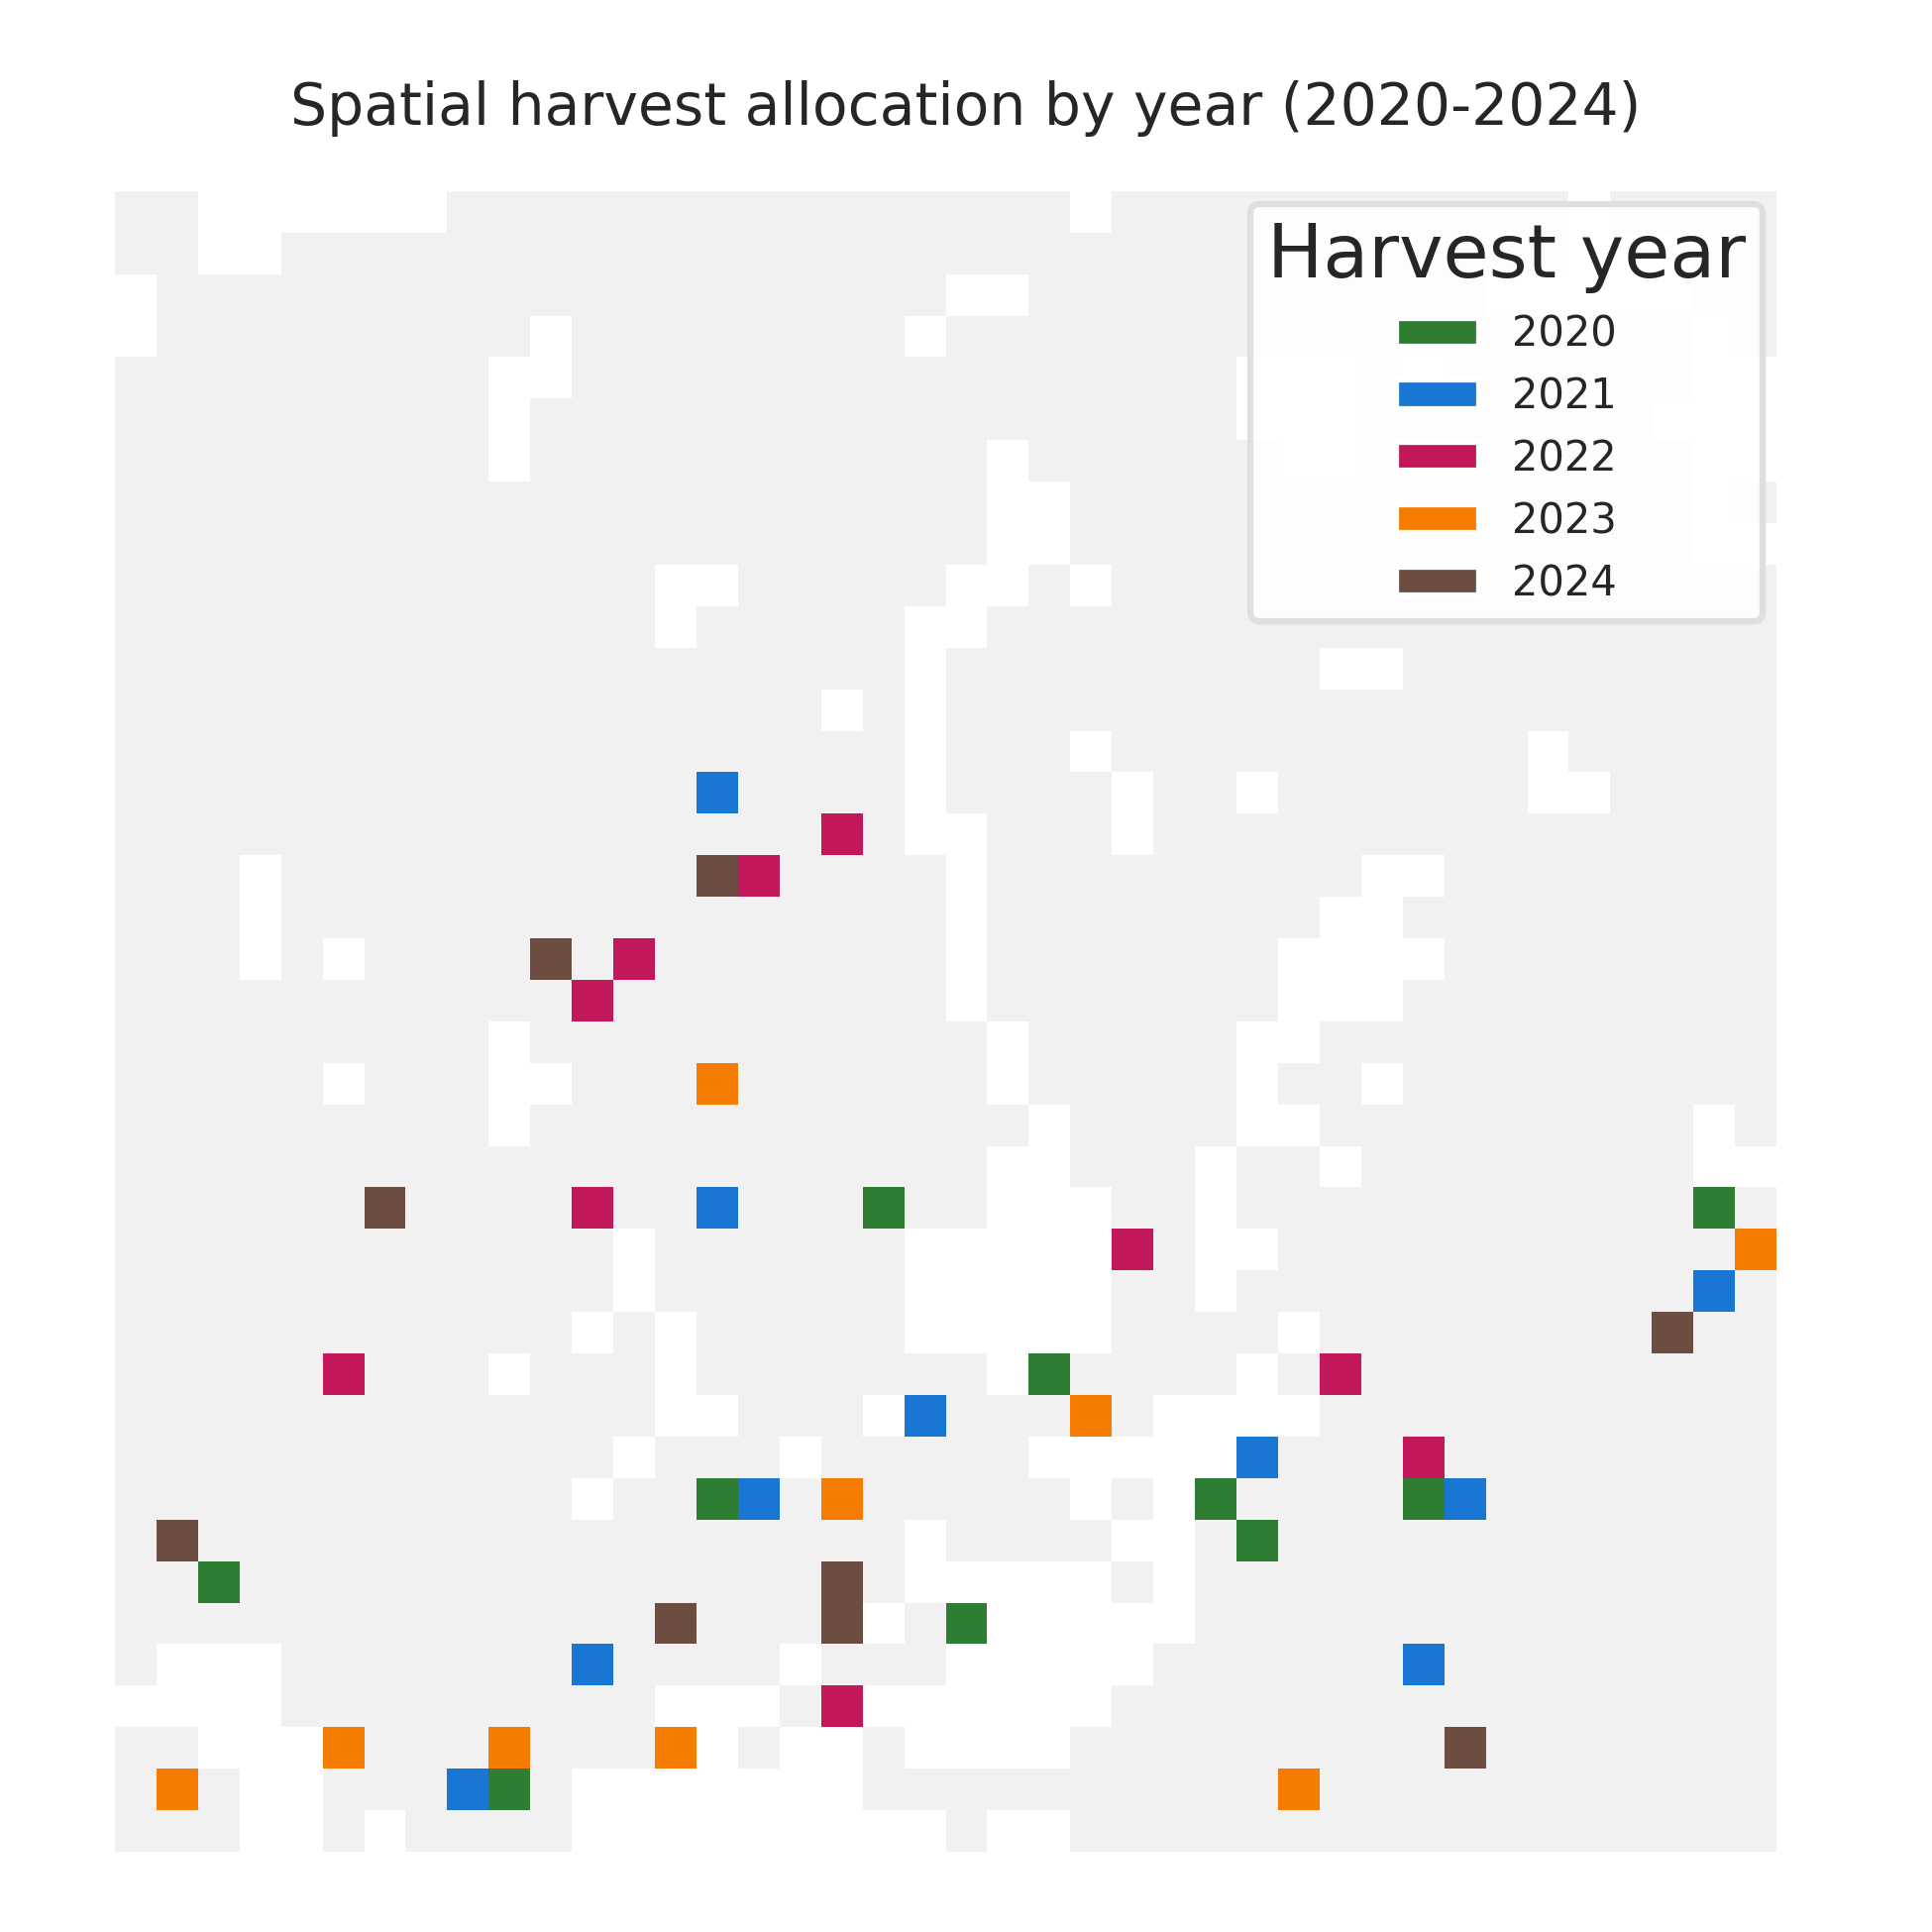
\includegraphics[width=0.7\linewidth]{figs/f3_spatial_allocation.png}
  \caption{Heuristic schedule allocated to space for the 2020--2024 planning window. Colours denote the first year a cell is harvested, overlaid on the full inventory extent (light grey).}
  \label{fig:spatial_allocation}
\end{figure}

WS3 delivers four primary contributions:
\begin{enumerate}[label=(\roman*)]
  \item A solver-agnostic, path-based Model~I generator embedded within an audited forest estate API, with parallel coefficient compilation for large instances.
  \item A first-class libCBM interface that exports Standard Input Tables and ingests carbon pools and fluxes for integrated mitigation accounting.
\item A hybrid aspatial-to-raster allocation workflow that emits reproducible geospatial artefacts from deterministic schedules.
  \item A FAIR-aligned reproduction package, including scaling benchmarks on real inventories and archived releases with pinned environments.
\end{enumerate}

\FloatBarrier

\subsection{Optimization formulation (Model I)}
WS3 adopts a classic Model~I linear programming model formulation \citep{johnson1977techniques, gunn2007models} in which each decision variable selects the proportion of a development type (all stands with the same initial stratification variable values) allocated to a feasible root-to-leaf prescription (path) across the planning horizon. Let:
\begin{align*}
  I &: \text{ set of spatial zones (dtypes)} \\
  J_i &: \text{ set of feasible prescriptions (paths) for zone } i\in I \\
  O &: \text{ set of outputs (e.g., harvest area, harvest volume, growing stock, habitat)} \\
  O'&\subseteq O: \text{ targeted outputs subject to even-flow constraints} \\
  T &: \text{ set of planning periods} \\
  T'_p&\subseteq T: \text{ periods on which even-flow for output } p\in O' \text{ is enforced}
\end{align*}
Decision variables are proportions:
\[
x_{ij}\in[0,1] \quad \text{for all } i\in I,\, j\in J_i,
\]
meaning ``the fraction of zone $i$ assigned to prescription $j$''. Let $\mu_{ijot}$ denote the quantity of output $o\in O$ in period $t\in T$ produced by allocating $x_{ij}$ to path $j\in J_i$ for zone $i\in I$. Define a reference-period level $y_p:=\sum_{i\in I}\sum_{j\in J_i}\mu_{ijpt_p^R}x_{ij}$ for each targeted output $p\in O'$ at $t_p^R\in T$, and $\varepsilon_p$ as the allowable even-flow tolerance. With general lower/upper bounds $v^-_{ot},v^+_{ot}$ on outputs, the Model~I LP is:
\begin{align}
\text{maximize}\quad
& \sum_{i\in I}\sum_{j\in J_i} c_{ij}\,x_{ij} \label{eq:ws3_obj}\\
\text{subject to}\quad
& (1-\varepsilon_p)\,y_p \le \sum_{i\in I}\sum_{j\in J_i}\mu_{ijpt}\,x_{ij} \le (1+\varepsilon_p)\,y_p, && \forall p\in O',\, \forall t\in T'_p \label{eq:ws3_evenflow}\\
& v^-_{ot} \le \sum_{i\in I}\sum_{j\in J_i}\mu_{ijot}\,x_{ij} \le v^+_{ot}, && \forall o\in O,\, \forall t\in T \label{eq:ws3_bounds}\\
& \sum_{j\in J_i} x_{ij} = 1, && \forall i\in I \label{eq:ws3_coverage}\\
& 0 \le x_{ij} \le 1, && \forall i\in I,\, \forall j\in J_i. \label{eq:ws3_box}
\end{align}
The objective coefficients $c_{ij}$ encode the user-defined value of a path (e.g., total or discounted volume, revenues, multi-criteria scores). Constraints (\ref{eq:ws3_evenflow}) enforce even-flow on targeted outputs, (\ref{eq:ws3_bounds}) set general lower/upper bounds per period, (\ref{eq:ws3_coverage}) ensures convex mixing of paths to fully cover each zone, and (\ref{eq:ws3_box}) bounds variables as proportions. In WS3, $\mu$-coefficients arise from replaying each path through the simulator, calling \texttt{compile\_product} (for action-dependent outputs like harvest area/volume) or \texttt{inventory} (for stocks like growing stock). The LP matrix is extremely sparse because each path contributes to a limited set of outputs and periods.

\emph{Code-to-math mapping.} WS3 exposes a coefficient-function pattern that compiles objective and constraint rows from paths. For example, helper functions like \texttt{cmp\_c\_z} (objective), \texttt{cmp\_c\_caa} (action-based flows), and \texttt{cmp\_c\_ci} (inventory-based constraints) traverse path nodes (period, action code, dtype key, age), evaluate the corresponding $\mu$-like contributions via \texttt{compile\_product}/\texttt{inventory}, and assemble the LP using \texttt{fm.add\_problem(...)}. Users select the solver (HiGHS by default; Gurobi optional) and solve via the standard PuLP interface. Upon optimality, WS3 compiles and applies the schedule, then re-simulates to produce indicators for analysis.

\emph{Design implications.} This path-based Model~I approach embeds intertemporal feasibility in each column, separates simulation from optimization, and enables straightforward addition of new outputs/constraints by supplying new coefficient functions. It also aligns with established forest-planning literature while remaining solver-agnostic and highly sparse for scalability.

\subsection{Implementation} 
\emph{Technology stack.} WS3 is implemented in Python and distributed via PyPI. Optimization problems are formulated by WS3 and solved with the  open-source HiGHS \citep{highs} solver by default, with optional PuLP \citep{pulp} (for flexibility) and Gurobi \citep{gurobi} (for performance) bindings. Geospatial I/O uses rasterio/fiona/GeoPandas. Documentation (Sphinx) and continuous integration ensure API consistency, example executability, and unit testing.

\emph{libCBM integration.} The ForestModel class exposes a \texttt{to\_cbm\_sit} method that compiles a CBM Standard Input Table (SIT) configuration and table data structure (i.e., classifiers, inventory, yields, disturbance events, transitions) consumable by libCBM. Users provide a disturbance type mapping and last-pass disturbance metadata to ensure correct dead organic matter (DOM) spin-up. The sequential demonstration runs libCBM for 200 years using the official Python API and documentation \citep{libcbm_py_docs, libcbm_py_repo}.

\emph{Reproducibility and packaging.} The repository includes examples and a reproduction package (papers/ems/repro) with pinned requirements and scripts to generate all figures and tables. Versioned releases are archived on Zenodo \citep{ws3_zenodo2025}. WS3 supports interactive (via Jupyter notebooks) and batch (via Python shell scripts) workflows, or it can be embedded into or called from other software systems (like any other open Python package).

\subsection{Quality assurance and benchmarking}
\emph{Automated testing.} WS3 ships with a pytest suite that exercises the common, core, financial, forest, and optimization modules (29 tests). The suite runs in approximately 4~s on a Linux workstation (Python~3.12) and is executed for every push and pull request via a GitHub Actions workflow (Ubuntu, Python~3.10) that also regenerates a coverage badge \citep{ci_workflow}. Style tooling (black, ruff) is bundled in \texttt{requirements-dev.txt} and wired into the development makefile, ensuring consistent formatting before release.

\emph{Input stewardship and validity.} WS3, like its Woodstock heritage, makes no assumptions about inventories, yields, operability, objectives, or constraints. The space of ``valid input'' is project- and policy-specific and inherently high dimensional; exhaustive auto-validation is out of scope. WS3 provides targeted checks in high-leverage paths (e.g., fallback to template transitions when age-specific rules are missing; basic range/shape sanity checks) and clear documentation of required structures for inventories, yields, actions, and transitions. Responsibility for input quality and modeling assumptions rests with qualified analysts; WS3 is a professional framework rather than a prescriptive application.

\emph{Determinism and reproducibility.} Given identical inputs, WS3 produces identical outputs. Minor nondeterminism is limited to optional solver seeds and randomized block ordering in the spatial allocation utility; both are controllable and fixed in the reproduction scripts. Consequently, statistical variance on deterministic time series is not meaningful; we report solved status, model scale, and runtime/throughput metrics instead. The reproduction package pins versions and seeds to yield byte-identical artifacts across runs, reflecting best practices for computational reproducibility \citep{peng2011reproducible}.

\emph{Verification against Woodstock.} WS3 was originally verified against Woodstock (2015) by replaying identical datasets and comparing action-specific flows and stocks across periods, yielding functionally equivalent outputs for the implemented subset of features. Known departures from Woodstock semantics are flagged in code and documentation. Ongoing development follows a trust-but-verify pattern: changes to core loops are regression-tested against known-good benchmarks before release.

\emph{Case-study repro checks.} The EMS reproduction package encapsulates the sequential WS3$\to$libCBM pipeline in \texttt{make\_repro.sh}. Inside the project’s reference LXD (Linux Containers) environment (Ubuntu~24.04 on dual Xeon~6254 CPUs, 72 logical cores, 768~GB PC-23400 RAM) the script completes in 6.1~s, re-creating Figures~\ref{fig:flows}--\ref{fig:cbm}, Figure~\ref{fig:spatial_allocation}, and the tables stored in \texttt{papers/ems/tables}. The workflow is deterministic: running \texttt{generate\_case\_study.py} a second time produces byte-identical CSV and PNG assets, providing an integration test for the scheduling, SIT export, and libCBM coupling.

\emph{Performance spot checks.} The heuristic scheduler used in the case study produces a 100-year plan in under a second, and the subsequent 200-year libCBM simulation dominates total runtime (\textasciitilde5~s). Larger linear programs formulated through \texttt{ws3.opt} benefit from HiGHS (default) or optional Gurobi: internal regression notebooks (e.g., Examples~030/040) routinely solve tens-of-thousands-of-stand path-based instances within minutes using HiGHS, while the optional Gurobi backend shortens solve time further via its advanced presolve and feasibility tools. Raster allocations scale linearly with the number of cells processed per period and are trivially parallelizable.

\emph{Optional scalability experiment.} To characterize scaling on real inventories, the reproduction package optionally integrates a DataLad-hosted benchmark dataset comprising five non-overlapping timber supply areas (TSAs) in northeastern British Columbia (the same study region as \citealt{boisvenue2022managing}). Enabling the optional step (\texttt{RUN\_SCALING=1}) fetches the dataset and executes \texttt{papers/ems/repro/run\_scaling\_benchmarks.py}, which sorts TSAs by complexity and evaluates them individually and cumulatively (\texttt{tsa08}, \texttt{tsa08+tsa40}, \ldots, \texttt{tsa08+tsa40+tsa41+tsa24+tsa16}). The scripted benchmark always runs the heuristic scheduler on a single worker---reflecting the implementation's serial design---and records sequential spatial-allocation runtimes using \texttt{ForestRaster}. On the reference container the heuristic schedules complete in 1.3--31.4~s while spatial allocation requires 46--656~s as problem size grows from 4.7~k to 37.7~k dtype--age pairs. Setting \texttt{RUN\_LP=1} extends the run to model-building benchmarks for the deterministic Model~I LP: WS3 constructs the LP with 1 and 16 workers (parallel coefficient compilation) and solves it with matching HiGHS thread counts, logging build/solve time, solver status, and stage-wise memory footprints. LP builds scale from 5.1~s (4.7~k dtype--age pairs) to 92.8~s (37.7~k dtype--age pairs) with single-worker compilation, while the 16-worker mode trims build time to 59~s at the cost of higher peak RSS (2.5~GB versus 1.8~GB). Because large path-based LPs routinely exceed tens of gigabytes of RAM on even larger inventories, the LP measurements are opt-in and intended for suitably provisioned systems. All metrics are written to \texttt{perf\_scaling.csv} with deterministic seeds so that regenerated figures and tables remain byte-identical; Figures~\ref{fig:scaling_sched}--\ref{fig:scaling_mem} and Table~\ref{tab:scaling_summary} summarise the resulting runtimes and memory profiles (Figures~\ref{fig:scaling_sched} and~\ref{fig:scaling_spatial}).

\begin{figure}[h]
  \centering
  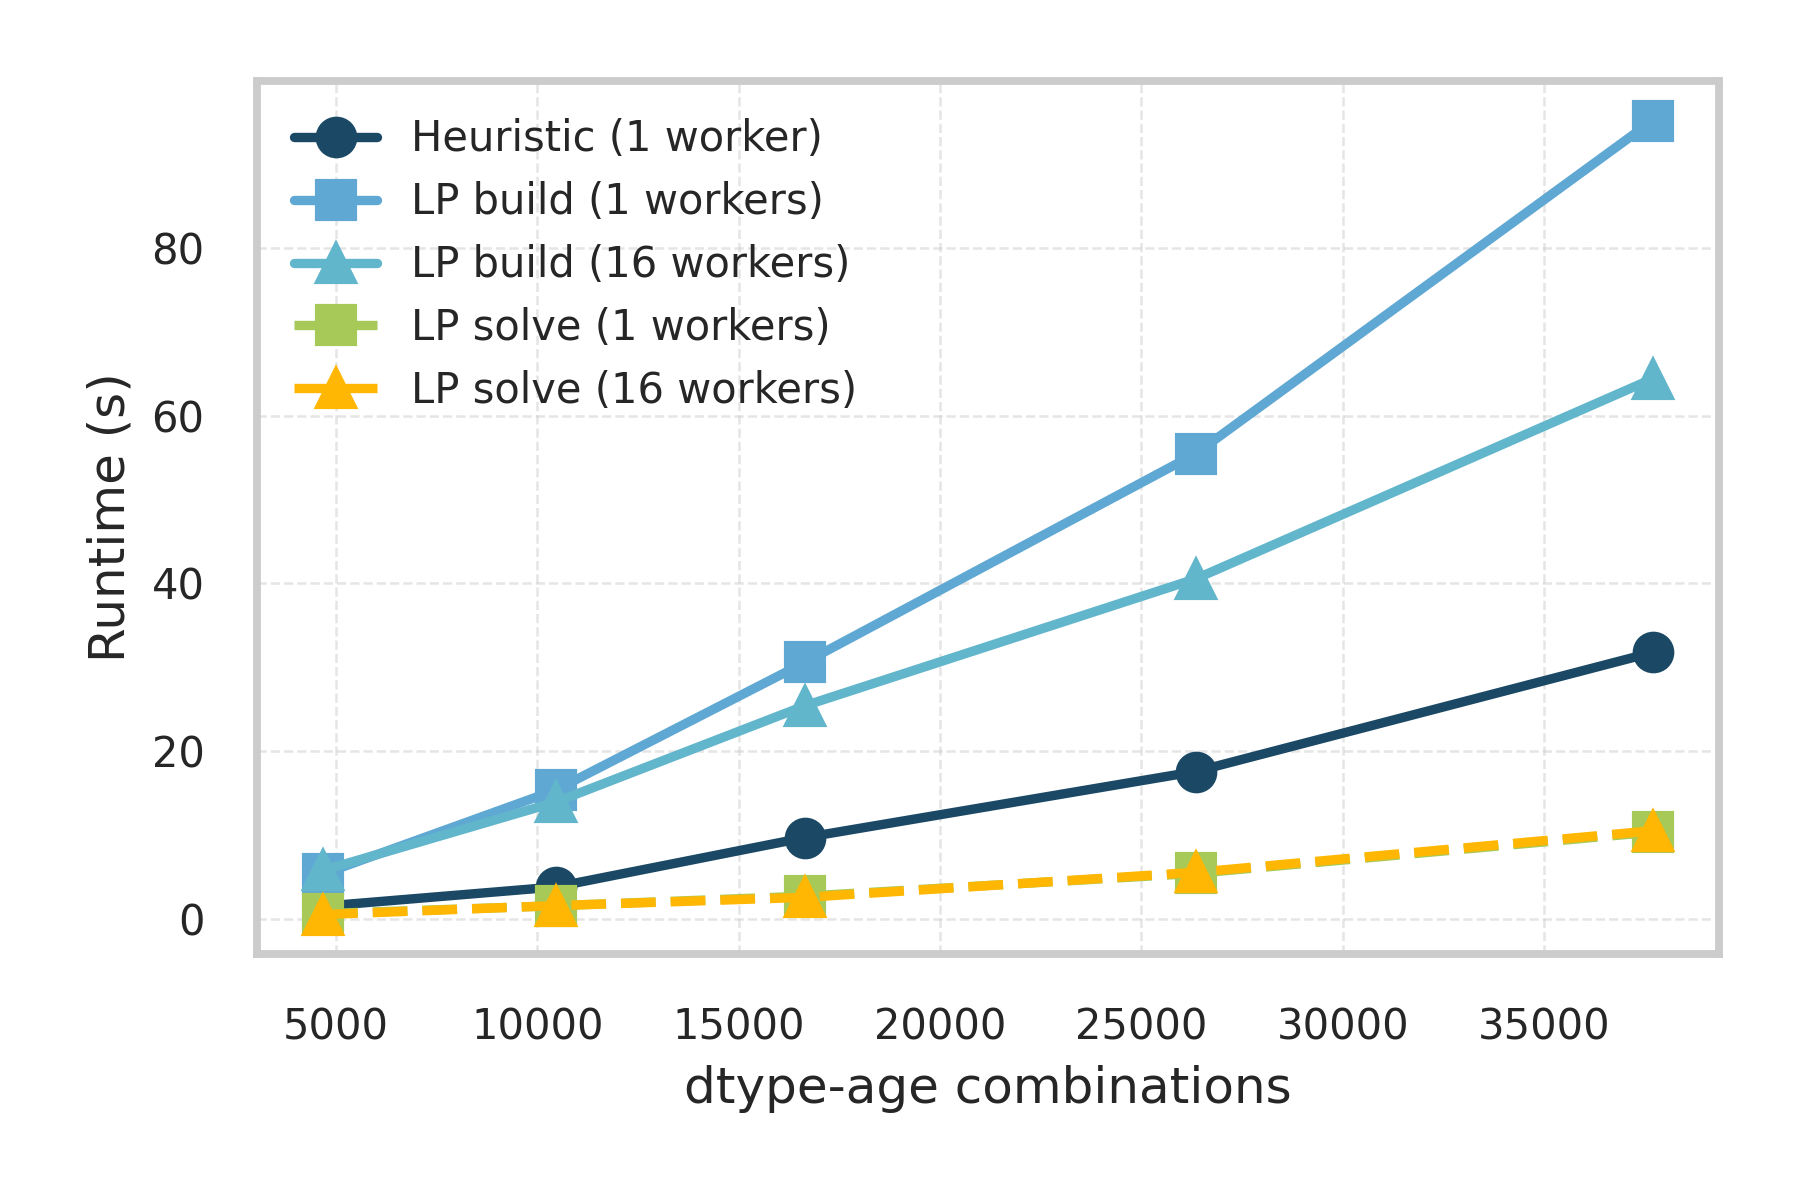
\includegraphics[width=0.85\linewidth]{figs/scaling_schedule_runtime.png}
  \caption{Scheduling runtime versus problem size, measured by the number of development type (dtype) by age combinations ($n_{\text{dtype-age}}$). Heuristic runs are single worker; LP build/solve lines appear when \texttt{RUN\_LP=1}.}
  \label{fig:scaling_sched}
\end{figure}

\begin{figure}[h]
  \centering
  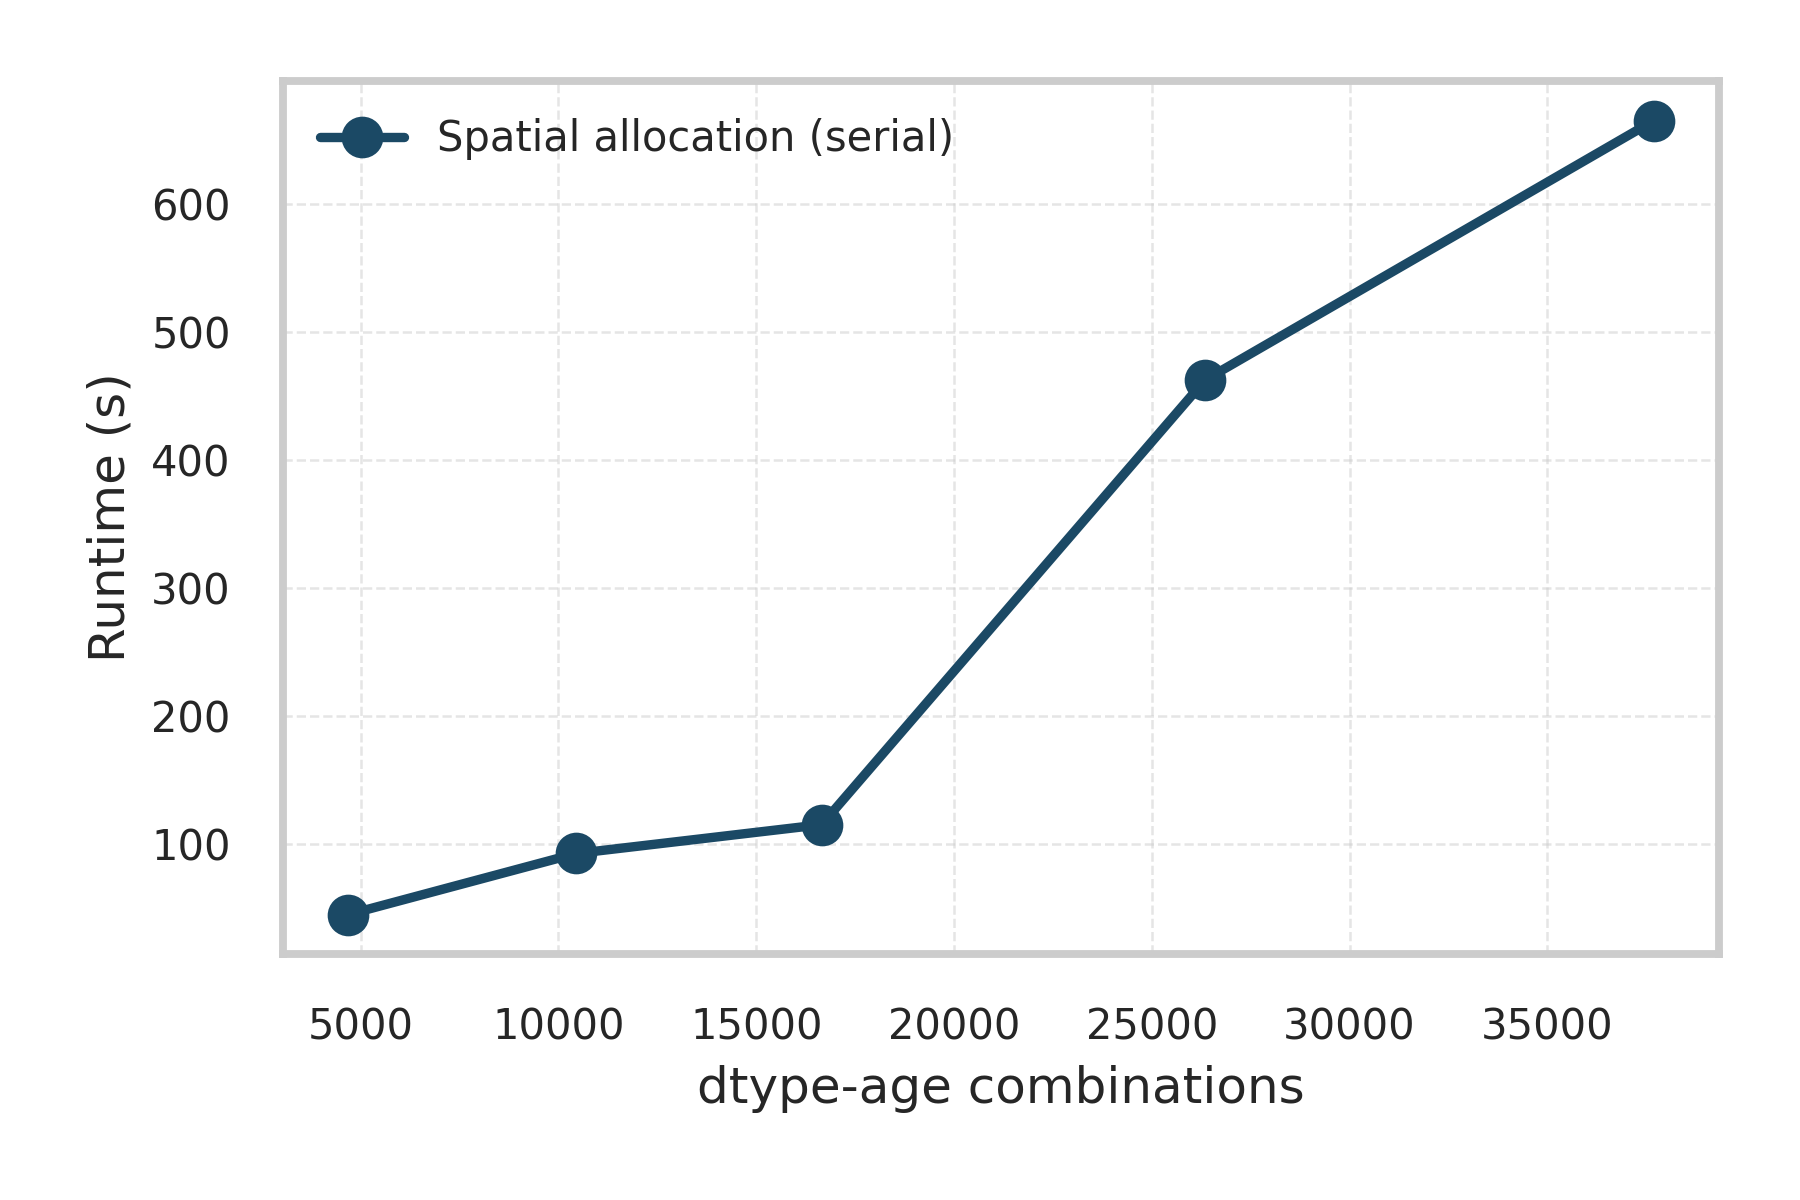
\includegraphics[width=0.85\linewidth]{figs/scaling_spatial_runtime.png}
  \caption{Spatial allocation runtime (serial \texttt{ForestRaster}) versus problem size after applying the heuristic schedule; problem size counts dtype--age combinations ($n_{\text{dtype-age}}$).}
  \label{fig:scaling_spatial}
\end{figure}

\begin{figure}[h]
  \centering
  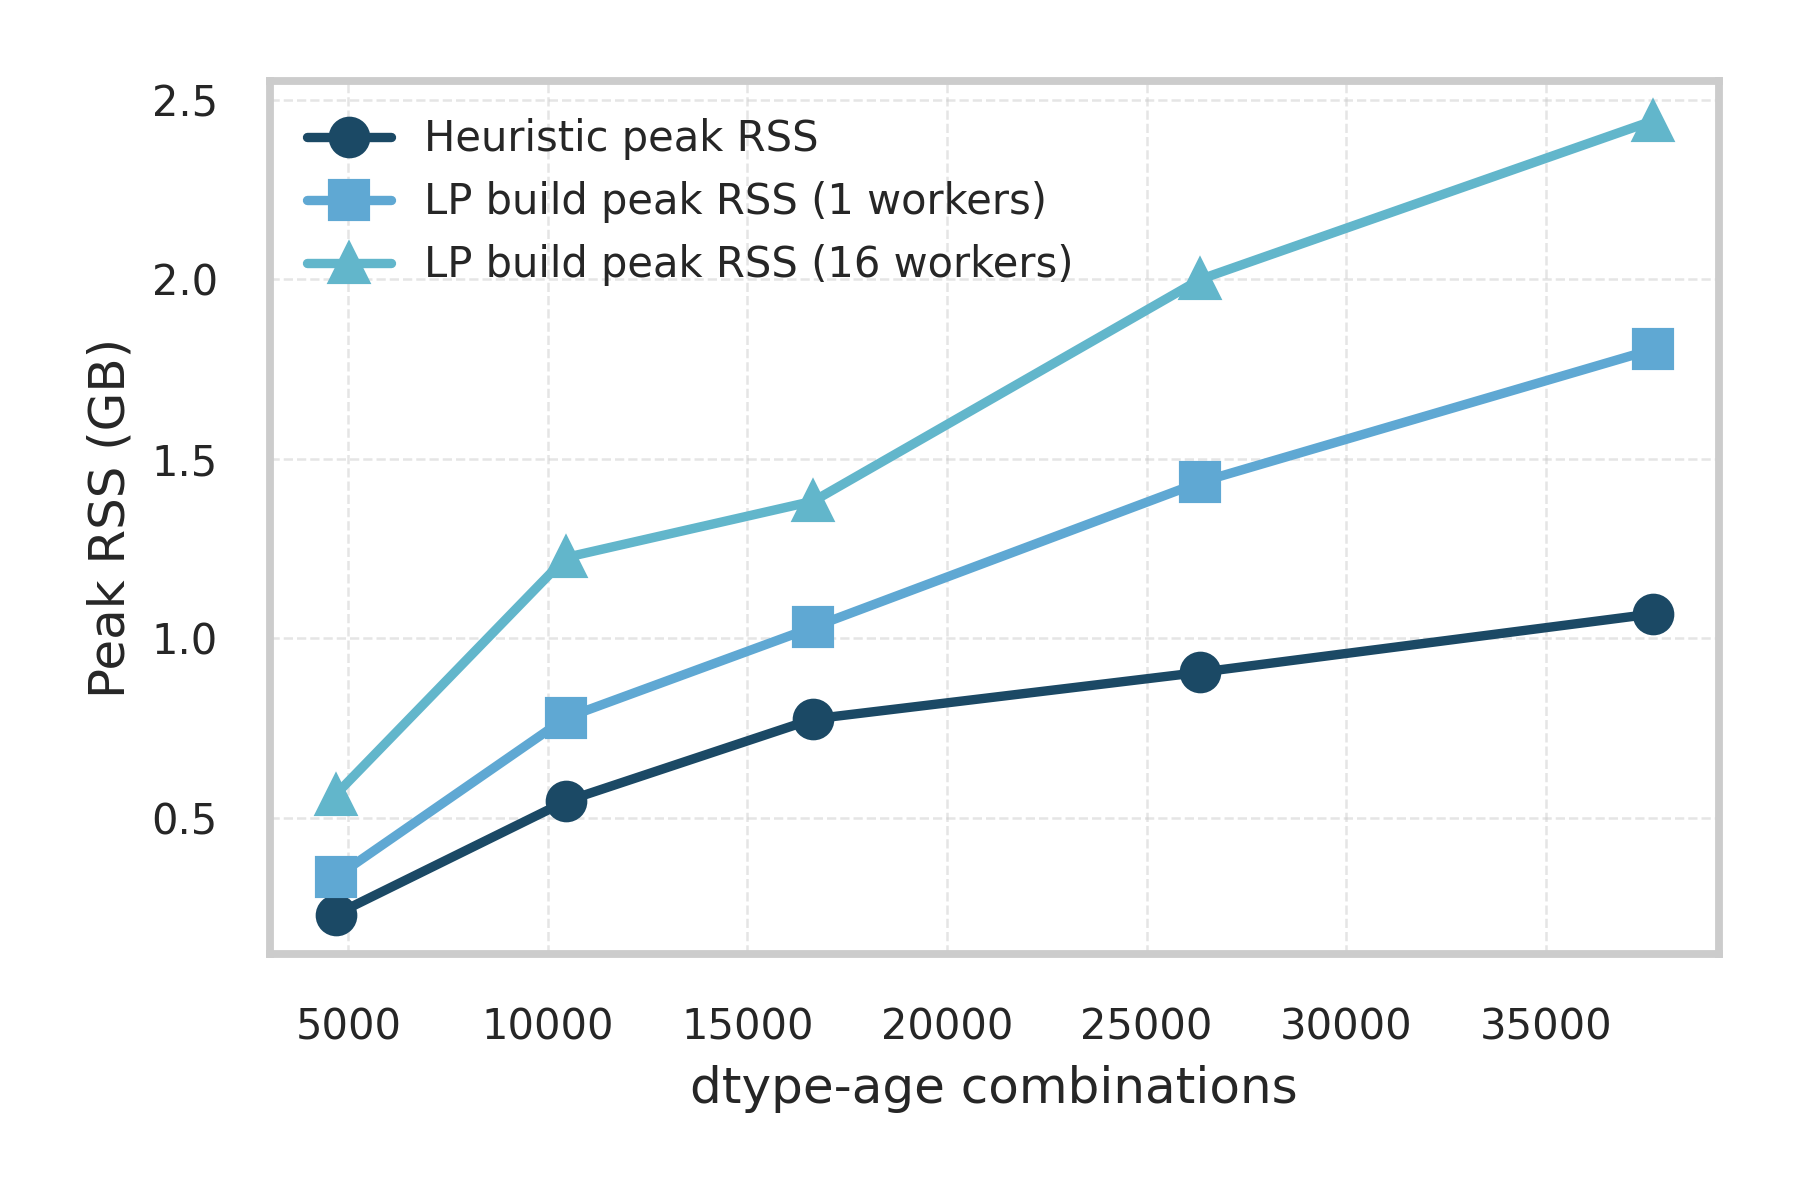
\includegraphics[width=0.85\linewidth]{figs/scaling_peak_mem.png}
  \caption{Peak resident memory for heuristic scheduling (serial) and LP model builds (1 and 16 workers) as problem size increases in terms of dtype--age combinations.}
  \label{fig:scaling_mem}
\end{figure}

\begin{table}[h]
  \centering
  \caption{Peak resident memory during heuristic scheduling and LP model builds on the reference container. $n_{\text{dtype-age}}$ counts development type (dtype) by age combinations; LP measurements report the maximum RSS observed while compiling the Model~I matrix with 1 or 16 workers, while spatial allocation runs serially.}
  \label{tab:scaling_summary}
  \begin{tabular}{lrrrr}
    \toprule
    Combo & $n_{\text{dtype-age}}$ & \shortstack[c]{Heuristic\\peak RSS\\(GB)} & \shortstack[c]{LP peak RSS\\(GB; 1 worker)} & \shortstack[c]{LP peak RSS\\(GB; 16 workers)} \\
    \midrule
    \texttt{tsa08} & 4\,682 & 0.23 & 0.33 & 0.56 \\
    \texttt{tsa08+tsa40} & 10\,453 & 0.52 & 0.78 & 1.22 \\
    \texttt{tsa08+tsa40+tsa41} & 16\,653 & 0.77 & 1.03 & 1.33 \\
    \texttt{tsa08+tsa40+tsa41+tsa24} & 26\,346 & 0.87 & 1.38 & 1.87 \\
    \texttt{tsa08+tsa40+tsa41+tsa24+tsa16} & 37\,691 & 1.07 & 1.81 & 2.51 \\
    \bottomrule
  \end{tabular}
\end{table}


\section{Illustrative use-case demonstrations}
\label{sec:usecase}
We open with a two-stage sequential pipeline demonstration that first schedules harvest in WS3 and then evaluates carbon dynamics using libCBM. The workflow replicates the existing example 031\_ws3\_libcbm\_sequential-builtin.ipynb to ensure full reproducibility.

\emph{Study design.} We use the public example dataset \texttt{tsa24\_clipped} provided with WS3. The inputs are stored as Woodstock-format text files (landscape, areas, yields, actions, transitions) under \path{examples/data/woodstock_model_files_tsa24_clipped} and imported into a \texttt{ForestModel}. We then schedule harvest using a self-parameterizing area-control heuristic to produce an aspatial action schedule over a 100-year horizon (10 periods of 10 years), and finally export a libCBM Standard Input Table (SIT) to simulate annual carbon stocks and fluxes.

\emph{Data and study area.} The \texttt{tsa24\_clipped} dataset is a clipped subset of a Timber Supply Area inventory used for demonstration. The initial inventory enumerates development types (dtypes) by theme tuples (e.g., analysis unit, species, site), with associated yield curves for total volume (\texttt{totvol}) and species-volume splits (\texttt{swdvol}, \texttt{hwdvol}). Actions and transitions define operability and state changes (e.g., harvest resets age).

\emph{Model setup and scheduling.} We initialize the model with \texttt{base\_year}=2020, \texttt{horizon}=10, \texttt{period\_length}=10\,y, and \texttt{max\_age}=1000. After importing sections and initializing areas, we add a null action and reset actions. The area-control scheduler selects target areas by mask (default: AU-wise THLB) and applies actions using a priority-queue selector (oldest-first). Target areas are computed from area-weighted mean CMAI ages; utilization is set to 0.85 in the volume expression used for compiled flows. The resulting schedule is compiled and applied to produce period-by-period flows and stocks.

\emph{libCBM coupling and metrics.} We define a disturbance-type mapping for actions (harvest$\to$Clearcut harvesting without salvage; fire$\to$Wildfire) and assign \texttt{last\_pass\_disturbance} per dtype to ensure consistent DOM spin-up. Using \texttt{ForestModel.to\_cbm\_sit} with softwood and hardwood volume names (\texttt{swdvol}, \texttt{hwdvol}), \texttt{admin\_boundary} = \texttt{"British Columbia"}, and \texttt{eco\_boundary} = \texttt{"Montane Cordillera"}, we export SIT config and tables. We then run libCBM for \texttt{n\_steps}=200 years, aggregating annual carbon stocks (biomass, DOM, total ecosystem).

\emph{Outputs.} We report time-series of harvested area/volume and growing stock from WS3, and annual carbon stocks from libCBM. The reproduction package generates the figures and tables used below.

The full, deterministic workflow is scripted in \texttt{papers/ems/repro/generate\_case\_study.py}, which produces the flows table and carbon stocks table:
\begin{itemize}
  \item \texttt{papers/ems/tables/scenario\_flows.csv}: harvest area, harvest volume, and growing stock by period.
  \item \texttt{papers/ems/tables/annual\_carbon\_stocks.csv}: annual biomass, DOM, and total ecosystem carbon.
\end{itemize}
\begin{table}[h]
\centering
\caption{Sequential demonstration parameters and configuration (WS3 $\to$ libCBM pipeline).}
\begin{tabular}{p{4.2cm}p{9.5cm}}
\toprule
Setting & Value \\
\midrule
Dataset & \texttt{tsa24\_clipped} (Woodstock-format inputs; \texttt{examples/data/woodstock\_model\_files}) \\
Base year & 2020 \\
Planning horizon & 10 periods (100 years) \\
Period length & 10 years \\
Max age class & 1000 years \\
Yield names & \texttt{totvol} (total volume), \texttt{swdvol} (softwood), \texttt{hwdvol} (hardwood) \\
Scheduling method & Area-control heuristic (priority-queue, oldest-first); utilization 0.85 \\
Disturbance mapping (CBM) & harvest$\to$Clearcut harvesting without salvage; fire$\to$Wildfire \\
CBM export & \texttt{ForestModel.to\_cbm\_sit} (admin: British Columbia; eco: Montane Cordillera) \\
CBM run length & 200 annual steps \\
Outputs & \texttt{scenario\_flows.csv} (period, harvest\_area\_ha, harvest\_volume\_m3, growing\_stock\_m3); \texttt{annual\_carbon\_stocks.csv} (annual pools) \\
\bottomrule
\end{tabular}
\label{tab:case_params}
\end{table}

Figures~\ref{fig:flows} and \ref{fig:cbm} visualize the resulting flows and carbon stocks. The entire pipeline, including the workflow overview (Figure~\ref{fig:workflow_overview}), workflow pseudocode (Listing~\ref{lst:workflow}), and the spatial allocation example (Figure~\ref{fig:spatial_allocation}), is reproducible via \path{papers/ems/repro/make_repro.sh}. The libCBM run length (200 years) matches the example and can be adjusted.

Unless stated otherwise, areas are reported in hectares (ha) and volumes in cubic metres (m$^3$).

\begin{figure}[h]
  \centering
  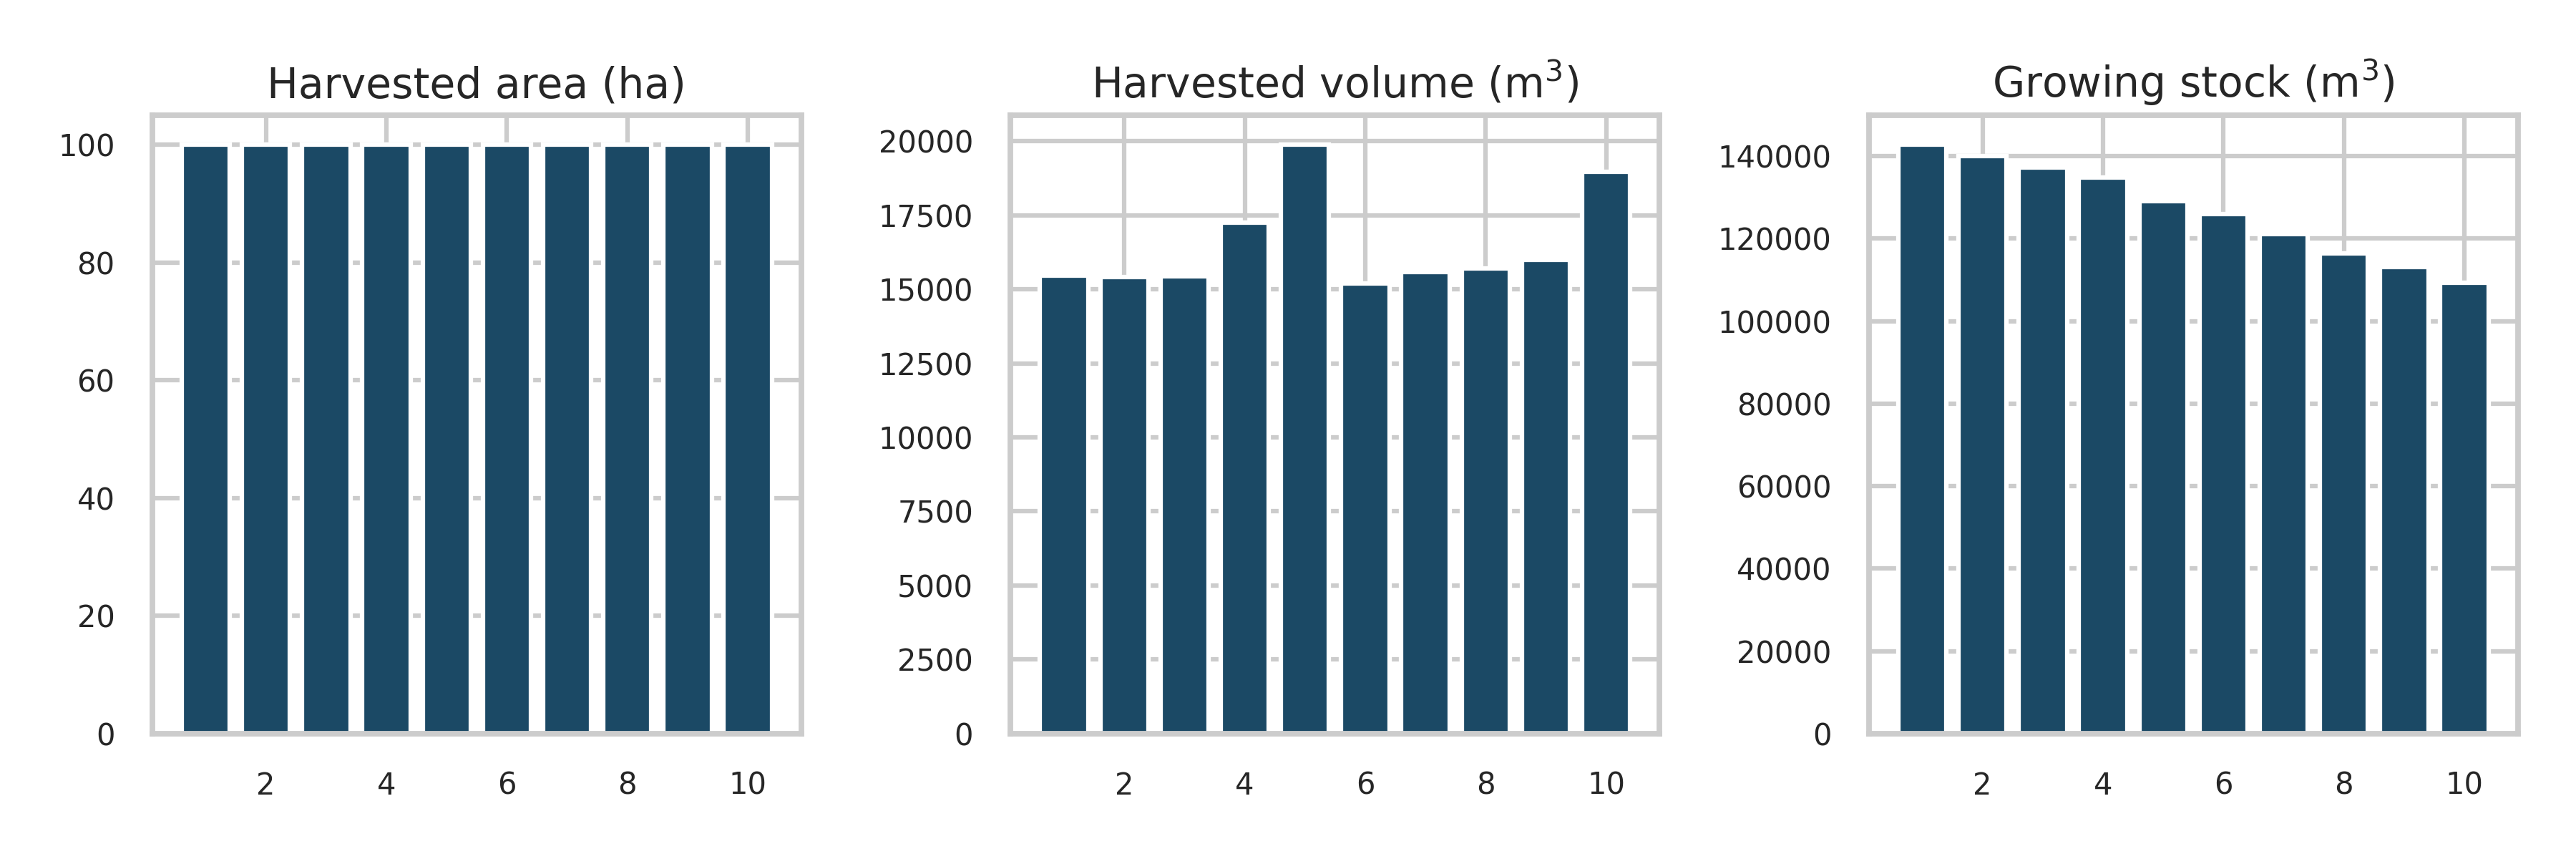
\includegraphics[width=0.95\linewidth]{figs/f4a_harvest_and_stock.png}
  \caption{WS3 results: harvested area, harvested volume (utilization-adjusted), and growing stock over planning periods.}
  \label{fig:flows}
\end{figure}

\begin{figure}[h]
  \centering
  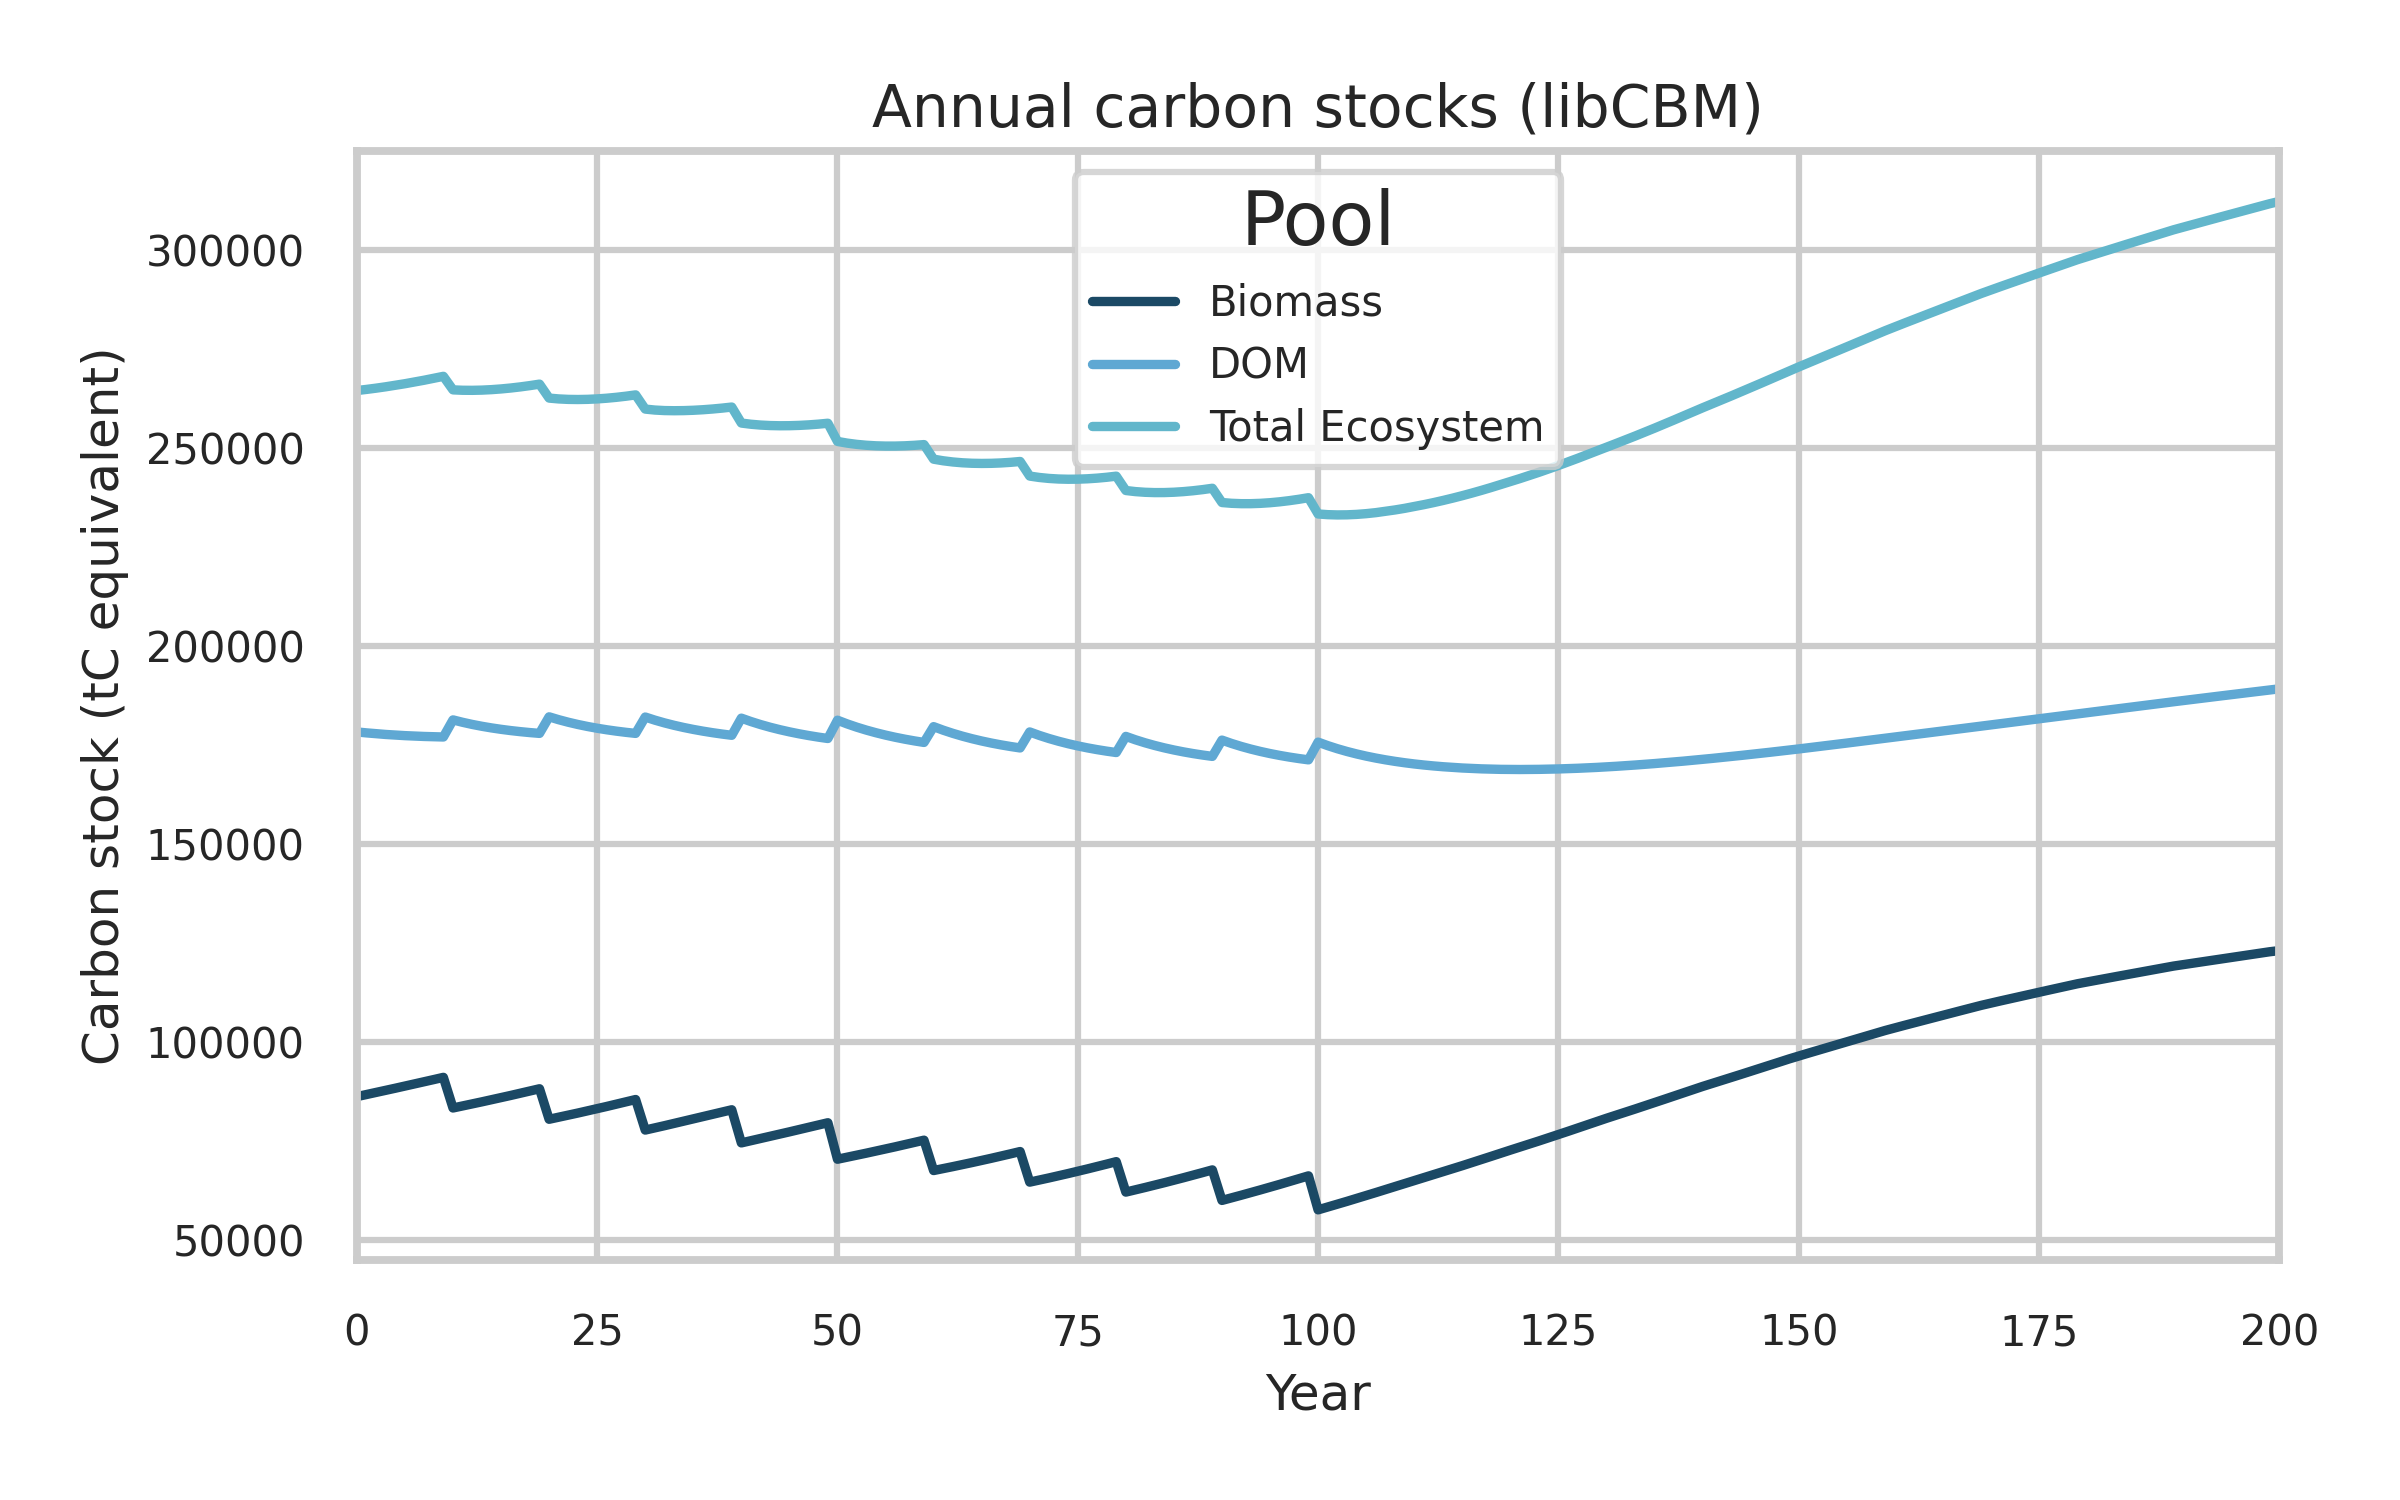
\includegraphics[width=0.95\linewidth]{figs/f4b_carbon_stocks.png}
  \caption{libCBM results: annual carbon stocks (biomass, dead organic matter, total ecosystem) over 200 years.}
  \label{fig:cbm}
\end{figure} 

\emph{Results.} The heuristic scheduler delivers a 10-period harvest plan whose flows stay within \textasciitilde10\% of their period means without any explicit even-flow constraint: harvest area averages 106.8~ha and ranges from 103 to 114~ha, while harvest volume averages 15.3~thousand~m$^3$ with a 14.1--18.5~thousand~m$^3$ span (Table~\ref{tab:case_params}; Figure~\ref{fig:flows}). Growing stock declines smoothly from 135~thousand to 82~thousand~m$^3$ (consistent with the 0.85 utilization factor), documenting the state trajectory exported to libCBM. In the carbon stage, libCBM aggregates show biomass pools increasing from $2.7\times10^5$~tC to $3.1\times10^5$~tC over 200 years, while DOM remains within $1.7$--$1.9\times10^5$~tC, yielding a total ecosystem carbon gain of 42~ktC (Figure~\ref{fig:cbm}). The summary tables \texttt{scenario\_flows.csv} and \texttt{annual\_carbon\_stocks.csv} (\texttt{papers/ems/tables}) retain the raw outputs for external verification.

\emph{Reproducibility.} This demonstration is intended to be transparent and portable; all input data reside in \path{examples/data/woodstock_model_files_tsa24_clipped}. The spatial allocation step renders the raster-based harvest allocation shown in Figure~\ref{fig:spatial_allocation}, derived directly from the aspatial schedule via the ForestRaster utility. The folder \path{papers/ems/repro} contains \path{make_repro.sh}, which provisions a clean virtual environment, installs pinned dependencies (including the optional libCBM extra via \texttt{pip install ws3[cbm]}), and runs deterministic scripts that regenerate Figures~\ref{fig:workflow_overview}--\ref{fig:cbm} and the accompanying CSV tables. Outputs are byte-identical on the reference container and stable under the pinned dependencies; the exact environment is preserved in the Zenodo-archived release.

\subsection*{Broader example library and carbon-aware optimization}
Beyond the sequential carbon-accounting demonstration, WS3 includes a curated set of executable notebooks designed as progressive tutorials, from synthetic examples to realistic policy-oriented analyses. Example 040 implements the classic Neilson hack from scratch and validates that aggregated WS3 carbon indicators closely track libCBM in a no-disturbance scenario. Carbon-aware optimization (embedding carbon prices/constraints directly in the LP and evaluating with \texttt{libcbm\_py}) is illustrated in Example 041. 
%A public, end-to-end use-case demonstration exploring carbon-aware scheduling in a stylized British Columbia landscape is available in the repository by Yan (MSc), including scenario automation, sensitivity analysis, and reproducible outputs \citep{yan2025mathematical, yan_repo}.

\begin{figure}[h]
  \centering
  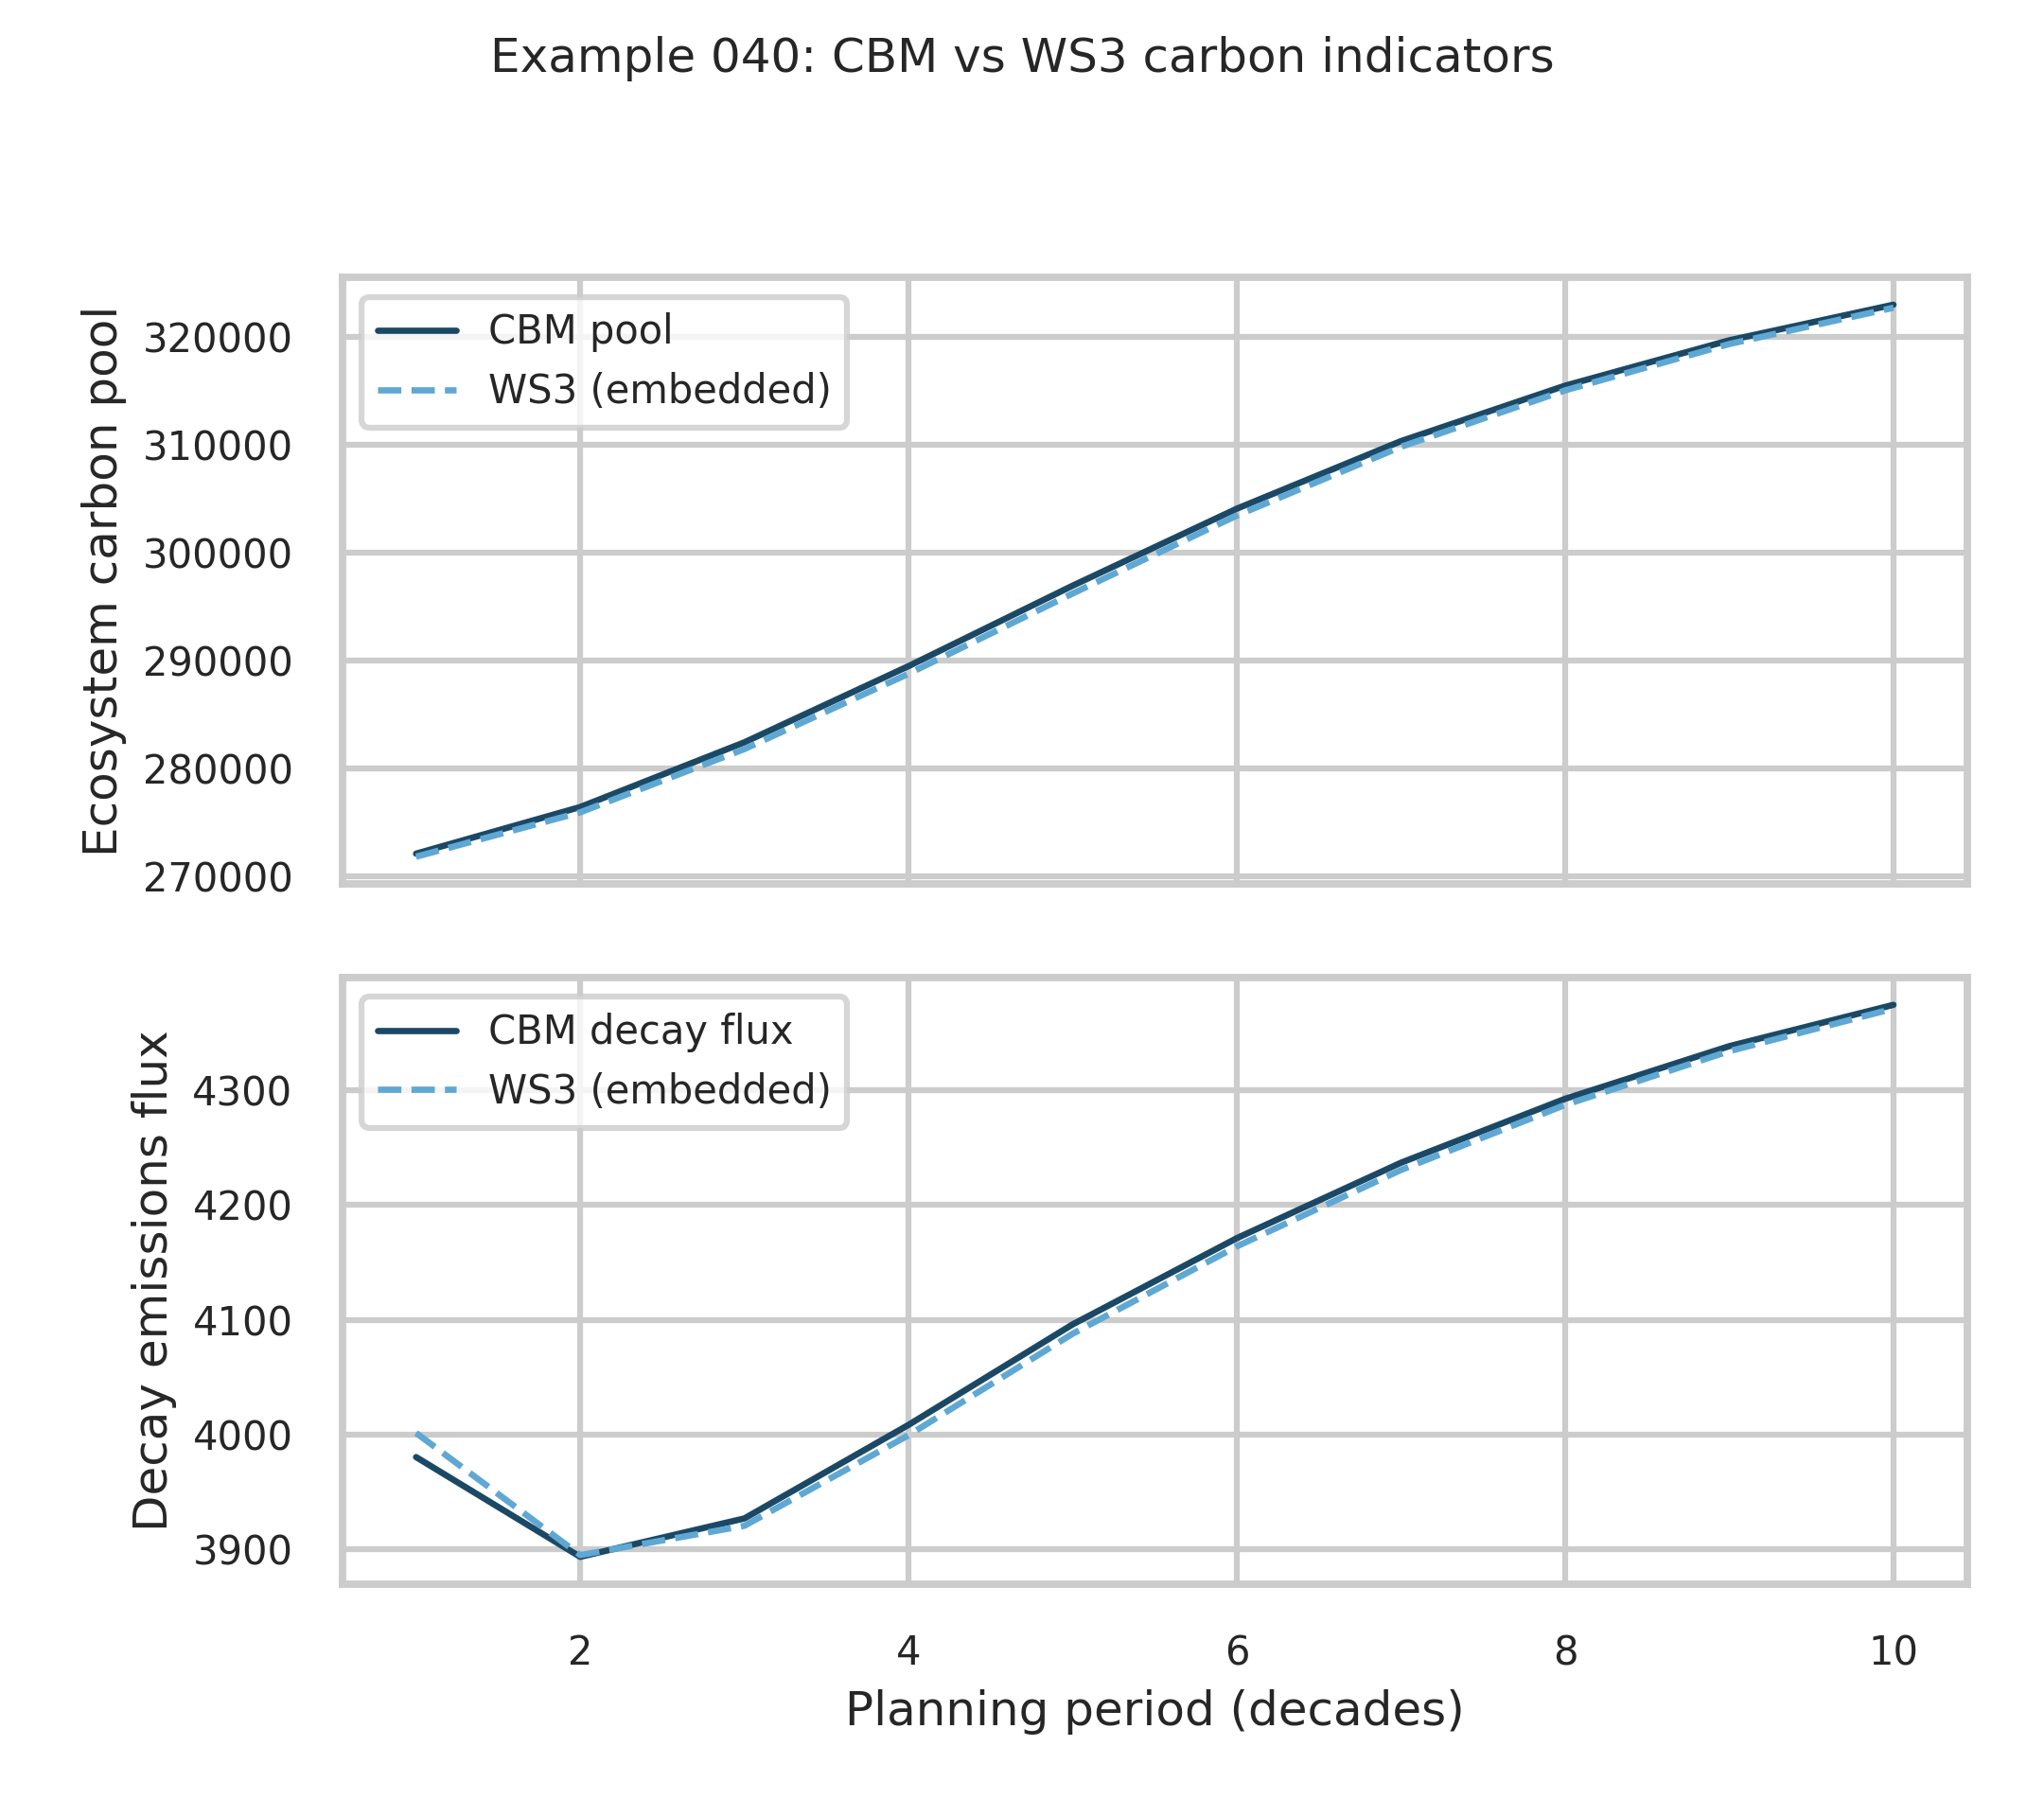
\includegraphics[width=0.95\linewidth]{figs/f5_neilsonhack_compare.png}
\caption{Neilson-hack demonstration (Example~040): comparison of libCBM (solid) and WS3-embedded (dashed) carbon indicators after bootstrapping pools/fluxes into WS3 as yield curves. Top: ecosystem carbon pools; Bottom: aggregate decay emissions flux. In a no-disturbance scenario, the aggregated indicators match closely; with harvesting, flux gaps reflect known limitations of the Neilson hack due to CBM DOM spin-up assumptions mapping time to age (Figure~\ref{fig:neilsonhack}).}
  \label{fig:neilsonhack}
\end{figure}

\section{Impact and reusability}

WS3 enables transparent, auditable analysis for forest landscape planning and climate mitigation, responding to calls for credible natural climate solutions and land-sector mitigation accounting \citep{griscom2017natural, gasser2020historical}. It has supported research on bioenergy \citep{cantegril2019bioenergy}, value-creation potential and supply modelling \citep{paradis2018retro, paradis2018estimating}, and climate impact assessment \citep{smyth2020climate, ke2024climate, yan2025mathematical}. WS3 integrates with the SpaDES ecosystem for spatial simulation \citep{spades} and has been deployed as a backend in decision-support applications. The open MIT license, modular API, and PyPI distribution lower barriers to community contributions and reuse across jurisdictions.

\paragraph{Major use-cases (2015--2025)}
\begin{itemize}
  \item Strategic wood supply and bioenergy planning in mixed-wood forests: optimization and scenario analysis of value-creation options \citep{cantegril2019bioenergy}.
  \item Hybrid simulation--optimization for value indicators and model retrofitting: methods and transfer to production-style analyses \citep{paradis2018retro, paradis2018estimating}.
  \item Climate mitigation and carbon-aware planning in British Columbia: sequential WS3$\to$libCBM pipelines and optimization under policy constraints; graduate theses and applied demonstrations \citep{ke2024climate, yan2025mathematical, yan_repo}.
  \item Decision-support prototypes for nature-based solutions: avoided fire and avoided harvest workflows (Examples 050/060) with net-emission indicators derived from libCBM.
  \item Integration with spatial simulation: \texttt{spades\_ws3} module bridging WS3 with SpaDES for disturbance and landscape dynamics studies \citep{spades, spades_ws3}.
  \item Application backends: WS3 used in web-based decision-support systems (e.g., \texttt{ecotrust-dss}) for scenario configuration and reporting \citep{ecotrust-dss}.
  \item Ongoing initiatives: CCCANDiES (integrated carbon and ecosystem services; in progress) and mining-sector nature-based solutions \citep{ghasemi2025decarbonization}. 
\end{itemize}

Interoperability fosters reusability: tabular/text inputs, raster outputs, and the libCBM linkage allow WS3 to slot into existing analytical pipelines. The reproduction package, unit tests, and continuous integration (CI) pipelines enhance trust and facilitate method transfer, aligned with community guidance on open and efficient scientific practice \citep{hampton2015tao, lowndes2017path}. The architecture is intentionally general, making it applicable to studies of sustainable yield, carbon accounting, biodiversity, and policy trade-offs \citep{boisvenue2022managing}.

\paragraph{Practical impact and reusability highlights}
\begin{itemize}
  \item Openness and packaging: MIT license, PyPI distribution, versioned releases archived on Zenodo \citep{ws3_zenodo2025}; complete examples and tutorials.
  \item Interoperability: Woodstock-format import for legacy/industry pipelines; libCBM SIT export for carbon; standard geospatial formats (GeoTIFF, shapefile).
  \item Reproducibility: deterministic reproduction package (\texttt{papers/ems/repro}) that regenerates all figures/tables; continuous integration (CI) runs tests and validates examples.
  \item Extensibility: modular API for adding outputs/constraints and new scheduling logic (heuristic or LP-based); solver-agnostic (HiGHS by default; Gurobi optional).
  \item Integration pathways: SpaDES ecosystem via \texttt{spades\_ws3}; backend for decision-support applications and web services.
  \item Education and onboarding: progressive example notebooks (from \texttt{010} to \texttt{060}) facilitate training and method transfer.
\end{itemize}

An advanced example notebook demonstrates how WS3 can be used to construct a stand-level optimization problem with explicit integration of carbon dynamics using \texttt{libcbm\_py}. This example solves a linear program that balances timber harvest revenues with carbon sequestration benefits under different carbon pricing assumptions (see Example 040). The workflow illustrates how WS3’s optimization layer and libCBM coupling enable carbon-aware planning experiments without bespoke glue code, supporting emerging policy analyses in nature-based climate solutions.

\section{Comparison to alternatives}

\begin{table}[h]
  \centering
  \caption{Comparison of WS3 with selected tools.}
  \begingroup
  \setlength{\tabcolsep}{3pt}
  \renewcommand{\arraystretch}{0.92}
  \footnotesize
  \begin{tabular}{p{2.4cm}p{2.1cm}p{1.5cm}p{2.0cm}p{2.0cm}p{1.9cm}p{1.9cm}}
  \toprule
  Tool & Scope & License & Optimization & Spatial & Carbon & Region \\
  \midrule
  WS3 & Landscape & Open (MIT) & Built-in (PuLP; optional Gurobi) & Hybrid aspatial-to-raster & Built-in libCBM linkage & General \\
  Woodstock & Landscape & Proprietary & Built-in & Extensions; connectors & External integrations & General \\
  Patchworks & Landscape & Proprietary & Built-in & Spatial planning emphasis & External integrations & General \\
  SpaDES & Simulation framework & Open & External packages & Fully spatial (agent-based, raster) & Via modules & General \\
  SIMFOR & Stand-level & Open & Limited/none & N/A & Limited/none & General \\
  Heureka & Landscape & Restricted (mixed) & Built-in & Spatial capabilities & External integrations & EU-focused \\
  JLP (MELA) & Landscape & Restricted (legacy) & Built-in & Spatial extensions & External integrations & Finland-focused \\
  \bottomrule
  \end{tabular}
  \endgroup
\end{table}

\paragraph{Parity with Woodstock}
To reassure readers that WS3 implements standard inventory accounting correctly, we report a parity check against a prescriptive Woodstock run using the same toy dataset and an identical action schedule. The accompanying CSV artifact \path{papers/ems/tables/woodstock_parity.csv} provides total harvest area, harvest volume, and growing stock, along with WS3-relative percent differences (computed as $100\,(\mathrm{WS3{-}Woodstock})/\mathrm{Woodstock}$). For transparency, period-wise parity summaries for harvest area and volume can be regenerated via the reproduction scripts and are included in the reproduction package. (Figure~\ref{fig:sup_parity_periods}) Exact or near-exact agreement is expected given identical inputs.

\loadWoodstockParity
\begin{table}[h]
  \centering
  \caption{WS3 vs. Woodstock parity on the toy dataset (identical schedule). Values are loaded from the accompanying CSV artifact.}
  \label{tab:woodstock_parity}
  \footnotesize
  \begin{tabular}{lrrr}
    \toprule
    Metric & WS3 & Woodstock & WS3 vs Woodstock (\%) \\
    \midrule
    Total harvest area (ha) & 1,000.00 & 1,000.00 & 0.00 \\
    Total harvest volume (m$^3$) & 164,838.08 & 164,838.08 & 0.00 \\
    Total growing stock (m$^3$) & 1,269,692.15 & 1,269,692.15 & 0.00 \\
    \bottomrule
  \end{tabular}
\end{table}

\begin{figure}[htbp]
  \centering
  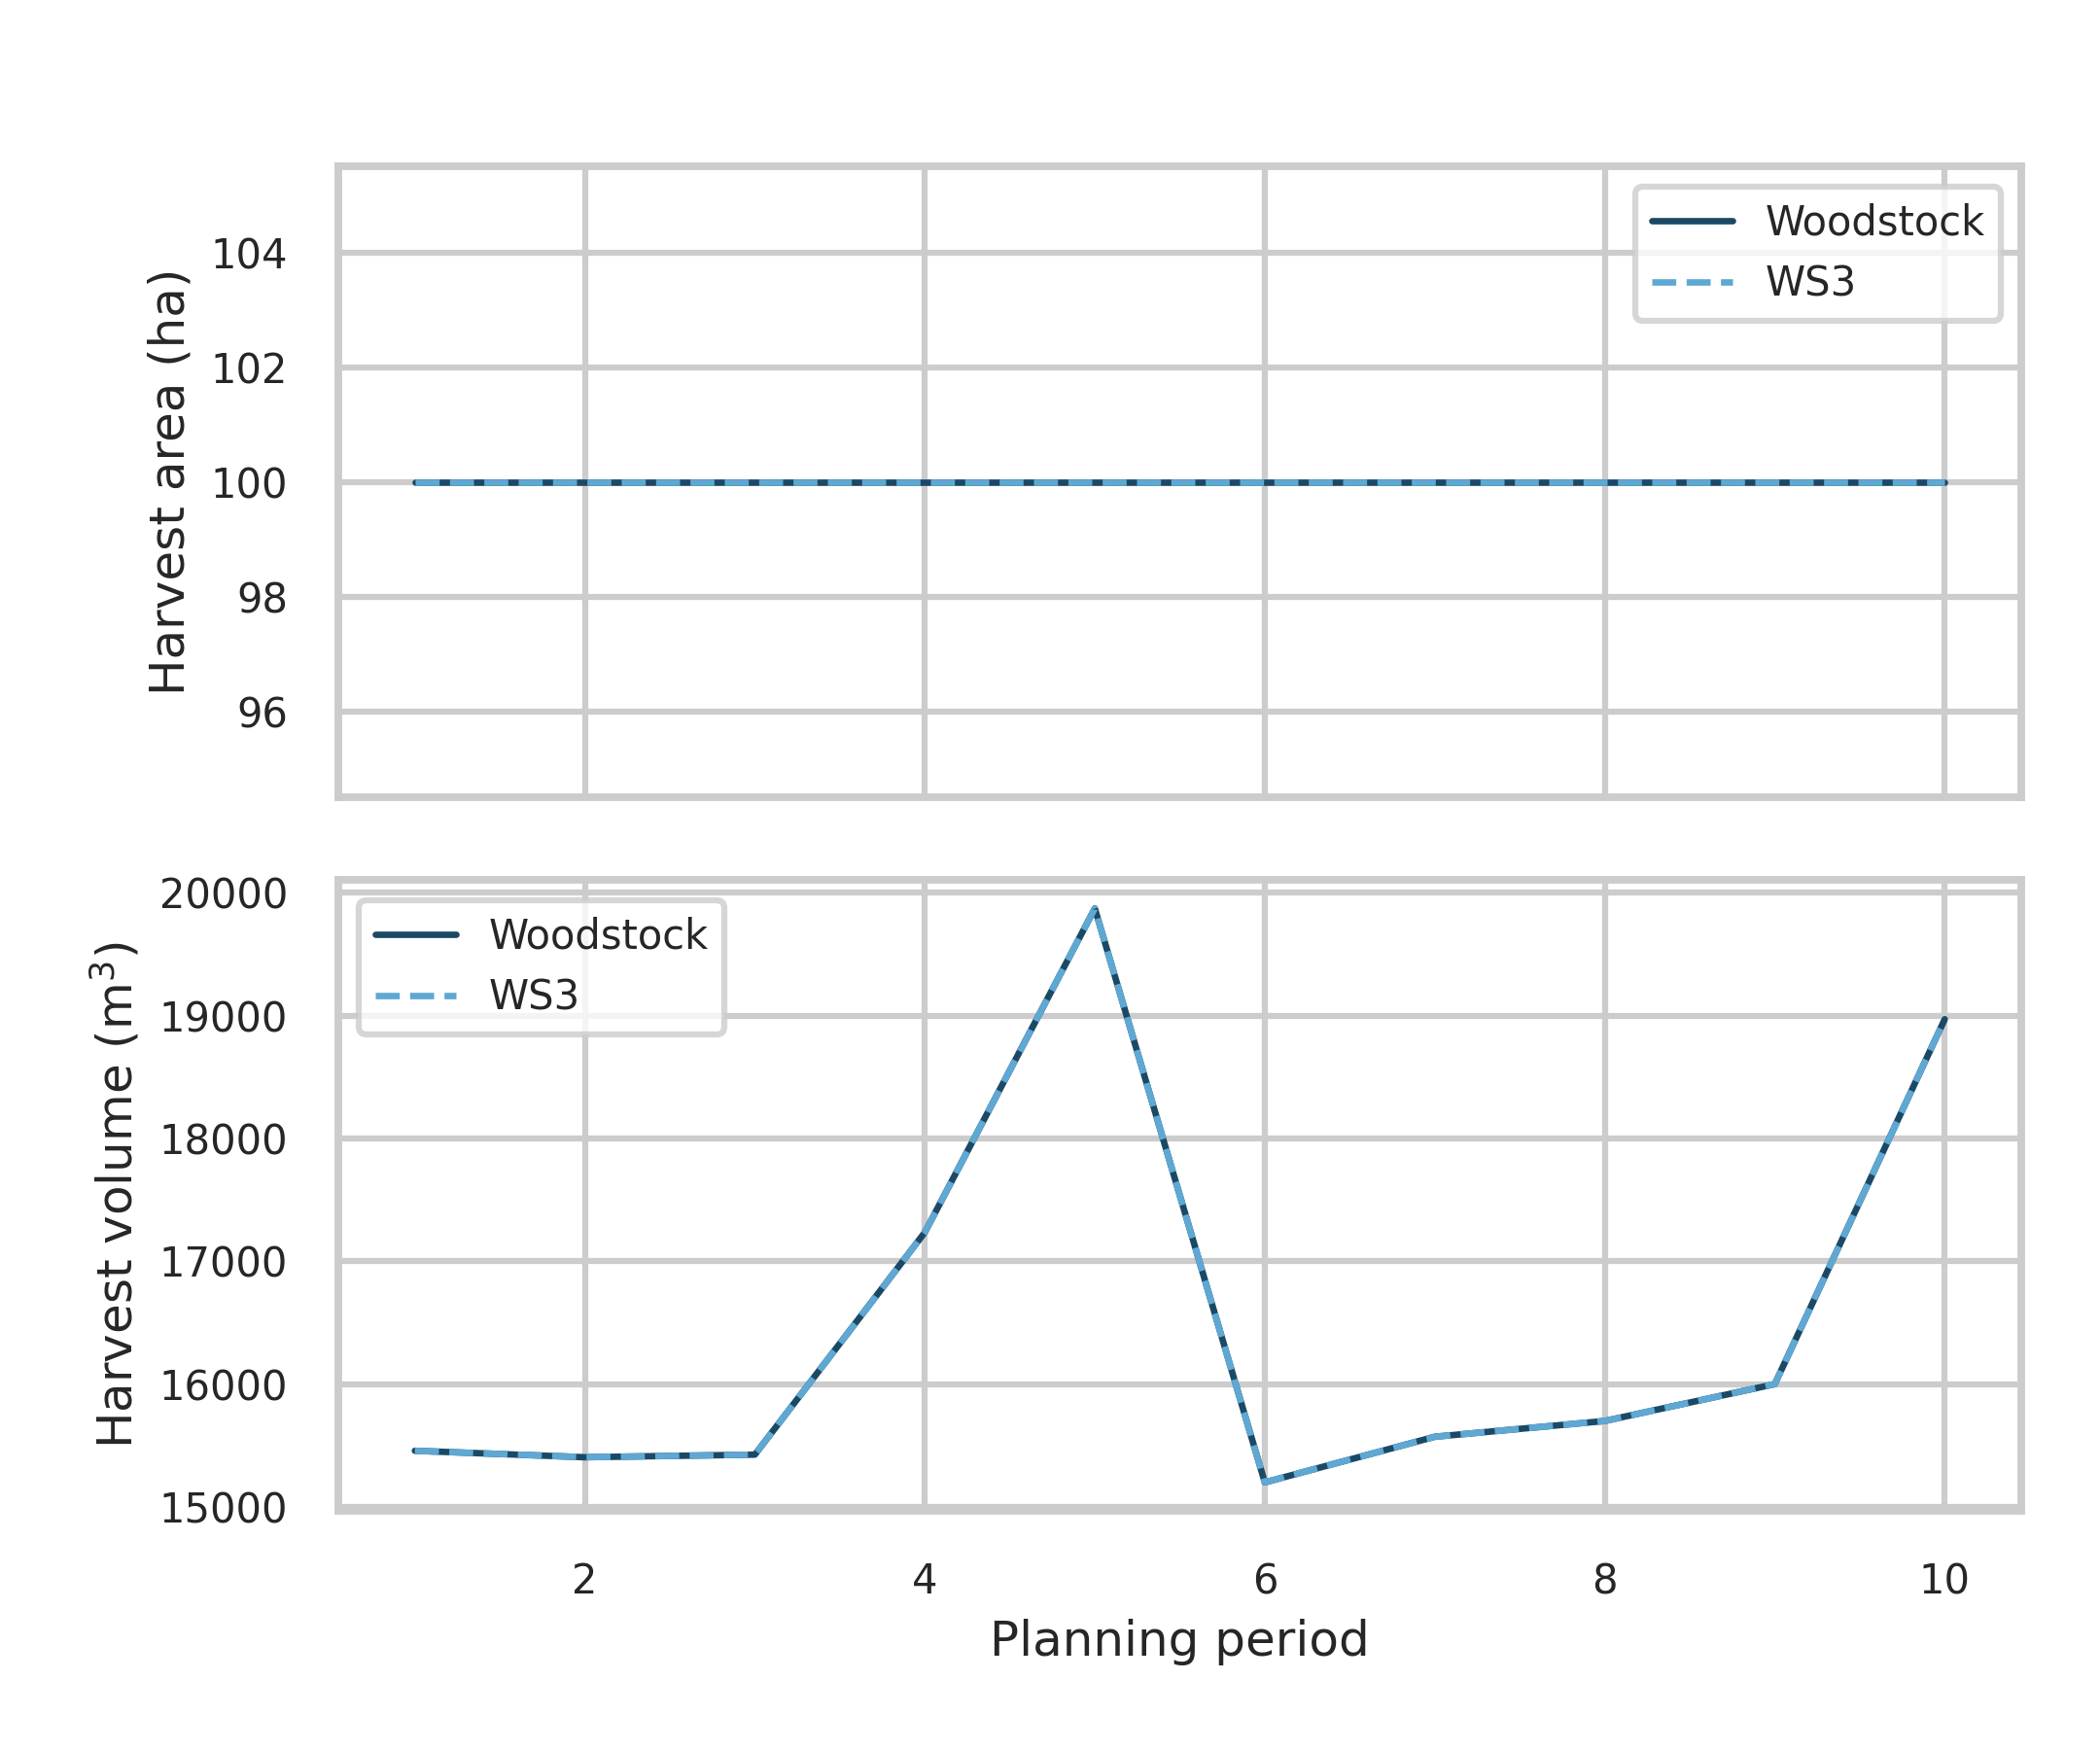
\includegraphics[width=0.95\linewidth]{figs/sup_parity_periods.png}
  \caption{Period-wise parity of harvested area and harvested volume between WS3 and Woodstock on the toy dataset (identical schedule). Values are loaded from the accompanying CSV artifact.}
  \label{fig:sup_parity_periods}
\end{figure}

\noindent
WS3 differs primarily in its open Python API, explicit libCBM integration, and hybrid spatial/aspatial workflow designed for reproducible research and policy analysis. We emphasize that SIMFOR operates at stand level, while WS3, Woodstock, Patchworks, Heureka, and JLP target landscape-scale planning with varying degrees of spatial explicitness and availability \citep{remsoft-woodstock, patchworks, spades, heureka, jlp_mela, simfor}.

\paragraph{Comparison narrative}
Proprietary landscape systems such as Woodstock and Patchworks provide mature optimization and spatial planning capabilities, but their licensing and closed codebases limit transparent methods development, automated testing, and reproducibility at scale. SpaDES, by contrast, is an open simulation framework oriented to spatial processes and agent-based dynamics; it does not natively provide a solver-backed harvest scheduling layer but interoperates with WS3 via \texttt{spades\_ws3} for hybrid workflows. Heureka and JLP are landscape-oriented and include optimization, yet are region-specific or legacy-maintained, which constrains adoption beyond their primary jurisdictions.

WS3’s distinctive contribution is to combine: (i) a solver-agnostic, path-based Model~I LP generator embedded directly in an open forest estate API; (ii) a documented, first-class linkage to libCBM for carbon stocks and fluxes; and (iii) a hybrid spatial/aspatial pipeline with standard geospatial I/O. These design choices enable reproducible, auditable workflows in notebooks and scripts, fast iteration on objectives/constraints, and easy integration into larger research and decision-support ecosystems. For many research and policy analyses, this balance of openness, extensibility, and end-to-end reproducibility is decisive—even when spatial planning itself is conducted in a specialized tool, WS3 can serve as the transparent scheduling and carbon accounting engine feeding it.

\section{Limitations and scope}
WS3 focuses on deterministic, aspatial forest estate formulations. The Model~I LP implementation is well suited to even-flow policies, policy bounds, and value-maximisation problems, yet it inherits the classic limitations of the formulation: stochastic or endogenous disturbances cannot be represented faithfully without departing from linearity, and non-linear objectives or constraints require either linearisation or external wrappers. In practice, we rely on the heuristic scheduler to interleave random disturbances or sensitivity analyses when scenario logic demands it, and reserve the LP for static policy experiments.

Spatial representation is delivered through a post-hoc raster allocation step that respects operability and transitions but does not enforce spatial adjacency, road-building, or block-shape constraints. Those dynamics fall outside the scope of WS3 and are the motivation for ongoing spatial extensions (e.g., the forthcoming WS4 prototype). Users requiring spatial optimisation should therefore treat WS3 as a scheduling and accounting engine that feeds specialised spatial tools.

Finally, large LP instances involve substantial memory pressure—tens of gigabytes for the largest benchmarks—because the column generation compiles full path matrices. The reproduction package flags the LP scaling experiment as opt-in so that teams can execute it on appropriately provisioned infrastructure. All supporting assets, however, remain deterministic and auditable even when the LP portion is skipped.

\section{Conclusions and future work}
WS3 provides an open, extensible framework for integrating harvest scheduling, simulation, and carbon accounting. By coupling solver-backed scheduling with libCBM via a documented interface, WS3 supports policy-relevant analyses with transparent, reproducible workflows.

Limitations of the current release centre on input data fidelity and computational resources. WS3 assumes that yield curves, transition rules, and carbon parameters supplied by users are defensible; errors in these inputs propagate directly into optimization outcomes and libCBM flux estimates. The deterministic Model~I formulation also omits stochastic disturbance processes and climate-forced growth uncertainty, so scenario ensembles are still required to bracket plausible futures. Finally, large linear programs can demand tens of gigabytes of memory and access to multi-core CPUs; while the reproduction package identifies these hotspots, practitioners should budget HPC or cloud resources accordingly.

Future work will expand uncertainty handling (stochastic scheduling, sensitivity analysis), add cloud/HPC deployment patterns, and strengthen spatial allocation and visualization. We also plan to enhance carbon–economics linkages and support machine learning surrogates for speedups in large scenario ensembles \citep{forrester2008surrogatemodelling}. The open design invites community extensions and cross-ecosystem applications.

\paragraph{Reproducibility}
All figures and tables are generated by scripts in \texttt{papers/ems/repro}. The \texttt{make\_repro.sh} script creates an isolated environment, installs pinned dependencies (\texttt{requirements.txt}), and runs \texttt{generate\_diagrams.py}, the spatial allocation workflow (\texttt{generate\_spatial\_allocation.py}), and the sequential demonstration script (\texttt{generate\_case\_study.py}). Outputs are written to \texttt{papers/ems/figs} and \texttt{papers/ems/tables}. The exact versions are preserved via the Zenodo-archived release.

\paragraph{FAIR compliance}
Table~\ref{tab:fair-checklist} summarises the EMS FAIR/software checklist submitted with the manuscript (see supplementary CSV \texttt{papers/ems/tables/fair\_checklist.csv}). WS3 remains Findable through its Zenodo DOI archive and indexed repositories, Accessible under the MIT license with public code/data artefacts, Interoperable via open tabular and geospatial formats plus Woodstock/libCBM linkages, and Reusable through pinned environments, continuous-integration (CI)–tested workflows, and full reproduction scripts \citep{ws3_zenodo2025}.

\begin{table}[h]
  \centering
  \caption{EMS FAIR/software checklist summary for WS3.}
  \label{tab:fair-checklist}
  \footnotesize
  \begin{tabular}{p{2.1cm}p{3.4cm}p{6.1cm}}
    \toprule
    Principle & Checklist focus & Evidence / artefact \\
    \midrule
    Findable & Persistent identifier; indexed repository & Zenodo DOI \href{https://doi.org/10.5281/zenodo.17331213}{10.5281/zenodo.17331213}; tagged GitHub releases; PyPI project metadata \\
    Accessible & License and public access & MIT license (CITATION.cff, LICENSE); public GitHub repository; PyPI wheels; reproduction package assets bundled in repository \\
    Interoperable & Open formats and connectors & Woodstock LAN/ARE/YLD importers; libCBM SIT export; tabular CSV, GeoTIFF, and shapefile outputs; documented workflow in Figure~\ref{fig:workflow_overview} \\
    Reusable & Documentation, provenance, validation & ReadTheDocs site; notebooks/examples; continuous-integration (CI)–tested \texttt{pytest} suite; deterministic scripts in \texttt{papers/ems/repro}; submission checklist metadata \\
    \bottomrule
  \end{tabular}
\end{table}

\section*{CRediT authorship contribution statement}
G.E.P.: Conceptualization, Methodology, Software, Validation, Formal analysis, Investigation, Data curation, Writing—original draft, Writing—review \& editing, Visualization, Supervision, Project administration, Funding acquisition.

\section*{Acknowledgements}
Development of WS3 was supported by the Forest Resources Environmental Services Hub (FRESH) at the University of British Columbia. The author thanks Elaheh Ghasemi, Salar Ghotb, and Kathleen Coupland for their contributions to documentation, testing, and code quality improvements leading up to this release. Language polishing and compliance checks were assisted by the OpenAI GPT-5 and GPT-5-Codex models; the author reviewed and edited all outputs.

\section*{Funding}
Funding: Natural Sciences and Engineering Research Council of Canada (NSERC, grant RGPIN-2023-04197); Environment and Climate Change Canada (ECCC, grant 3000770190); Natural Resources Canada (NRCan, grant 3000771054); Government of British Columbia (grant TP24FCCS004); Mitacs (Newmont Goldcorp Inc., grant IT32088).

\section*{Data availability}
Data availability: Source code, configuration files, and reproduction assets are archived at \href{https://doi.org/10.5281/zenodo.17331213}{https://doi.org/10.5281/zenodo.17331213}. All scripts used to generate the figures and tables are included; reuse is permitted under the MIT License.

\section*{Declaration of competing interest}
Competing interests: The author declares no competing interests.

\section*{Declaration of generative AI and AI-assisted technologies in the manuscript preparation process}
During the preparation of this work the author used the OpenAI GPT-5 and GPT-5-Codex models to assist with language polishing and format compliance. After using these tools, the author reviewed and edited the content as needed and takes full responsibility for the content of the published article.

\bibliographystyle{elsarticle-harv}
\bibliography{references}

\end{document}
